\chapter{Supplement for Bayesian Pseudocoresets}
\label{app:app1}
\renewcommand*{\MyPath}{../Appendix1}%

\section{Proof of~\cref{prop:original_coreset_fails}}
\label{app:proofs-of-failure}

In the setting of~\cref{prop:original_coreset_fails}, both the exact posterior and the coreset posterior 
are multivariate Gaussian distributions, denoted as $\distNorm{\left(\mu_1, \Sigma_1\right)}$ and 
$\distNorm{\left(\mu_{w}, \Sigma_{w}\right)}$ respectively. 
The mean and covariance are
\[
\Sigma_{1}=\frac{1}{1+ N} I_d, \quad \mu_{1}=\Sigma_{1}\left( \sum_{n=1}^{N} X_{n}\right), 
\label{eq:exact_post}
\]
and
\[
\label{eq:coreset_post}
\hspace{-.3cm}\Sigma_{w}\!=\!\frac{I_d}{1+ \left(\sum_{n=1}^N w_n\right)}, 
\quad
\mu_{w}\!=\!\Sigma_{w}\left( \sum_{n=1}^{N} w_n X_{n}\right).
\]

\begin{proof}[Proof of~\cref{prop:original_coreset_fails}]
	By~\cref{eq:exact_post,eq:coreset_post}, 
	\begin{equation} \label{eq:KL_from_coreset_post_to_exact}
	\begin{aligned}
	\kl{\pi_{w}}{\pi}
	=& \frac{1}{2}\left[\log\frac{|\Sigma_{1}|}{|\Sigma_{w}|} - d + \tr\left( \Sigma_{1}^{-1}\Sigma_{w}\right) +  
	(\mu_{1} - \mu_{w})^T \Sigma_{1}^{-1}(\mu_{1} - \mu_{w})\right]\\
	=& \frac{1}{2} \left[ -d\log \left( \frac{1+ N}{1+ \sum_{n=1}^N w_n}\right) - d  + d \left( \frac{1+ N}{1+ \sum_{n=1}^N w_n}\right)
	+  (\mu_{1} - \mu_{w})^T \Sigma_{1}^{-1}(\mu_{1} - \mu_{w})\right].
	\end{aligned}
	\end{equation}
	Note that $\forall x > 0, x-1 \geq \log x$, implying that 
	$$ -d\log \left( \frac{1+ N}{1+ \sum_{n=1}^N w_n}\right) -d + d \left( \frac{1+ N}{1+ \sum_{n=1}^N w_n}\right) \geq 0.$$ 
	Thus, 
	\begin{equation} \label{eq:first_inequality}
	\kl{\pi_{w}}{\pi} \geq \frac{1}{2}(\mu_{1} - \mu_{w})^T \Sigma_{1}^{-1}(\mu_{1} - \mu_{w}).
	\end{equation}
	Suppose we pick a set $\mcI\subseteq[N]$, $\left|\mcI\right| = M$ of active indices $n$ where the optimal $w_n \geq 0$,
	and enforce that all others $n\notin \mcI$ satisfy $w_n = 0$.
	Then denoting
	\[
	Y = \left[X_n : n\notin \mcI\right] \in \reals^{d\times (N-M)}, \quad
	X = \left[X_n : n\in \mcI\right] \in \reals^{d\times M},
	\]
	we have that for any $w\in \reals_+^M$ for those indices $\mcI$,
	\[
	\kl{\pi_w}{\pi} 
	\geq & \frac{1}{2(N+1)}1^TY^TY1 
	+1^TY^TX\left(\frac{1}{N+1} - \frac{w}{1+1^Tw}\right)\\
	&+\frac{N+1}{2}\!\!\left(\frac{1}{N+1}\! -\! \frac{w}{1+1^Tw}\right)^T\!\!\!\!\!X^T\!X\!\left(\frac{1}{N+1} \!-\! \frac{w}{1+1^Tw}\right).
	\]
	Relaxing the nonnegativity constraint, replacing $w/(1+1^Tw)$ with a generic $x\in\reals^M$, and 
	noting that $X^TX$ is invertible almost surely when $M < d$,
	we can optimize this expression yielding a lower bound
	on the optimal KL divergence using active index set $\mcI$,
	\[
	\kl{\pi_{w^\star_{\mcI}}}{\pi} &\geq \frac{1^TY^T\left(I-X(X^TX)^{-1}X^T\right)Y1}{2(N+1)}.
	\]
	The numerator is the squared norm of $Y1$ minus its projection onto the subspace spanned by the $M$ columns of $X$.
	Since $Y1 \dist \distNorm(0, (N-M)I)$, $Y1 \in \reals^d$ is an isotropic Gaussian, then its projection into the orthogonal
	complement of any fixed subspace of dimension $M$ is also an isotropic Gaussian of dimension $d-M$ with the same variance.
	Since the columns of $X$ are also independent and isotropic, its column subspace is uniformly distributed.
	So therefore, for each possible choice of $\mcI$
	\[
	\kl{\pi_{w^\star_{\mcI}}}{\pi} &\geq \frac{N-M}{2(N+1)} Z_{\mcI},  \quad Z_{\mcI}\dist \chi^2(d-M).
	\]
	Note that the $Z_\mcI$ will have dependence across the $N\choose M$ different choices of index subset $\mcI$.
	Thus, the probability that \emph{all} $Z_{\mcI}$ are large is
	\[
	\Pr\left(\min_{\mcI \subseteq [N], |\mcI| = M} Z_{\mcI} > \epsilon\right) 
	\geq &1 - {N\choose M}\Pr\left(Z_{\mcI} \leq \epsilon\right)\\
	= &1 - {N\choose M}F_{d-M}(\epsilon),
	\]
	where $F_{k}$ is the CDF for the $\chi^2$ distribution with $k$ degrees of freedom.
	The result follows.
\end{proof}


\section{Gradient derivations}
\label{app:gradient_derivations}

Throughout, expectations and covariances over the random parameter $\theta$ with 
no explicit subscripts are taken under pseudocoreset posterior $\piuw$. We also
interchange differentiation and integration without explicitly verifying that 
sufficient conditions to do so hold.

\subsection{Weights gradient}
\label{app:weights_gradient}

\setlength{\belowdisplayskip}{8pt} \setlength{\belowdisplayshortskip}{8pt}
\setlength{\abovedisplayskip}{8pt} \setlength{\abovedisplayshortskip}{8pt}
\allowdisplaybreaks

First, we compute the gradient with respect to weights vector $ w\in\reals^{M}_{+}$, which is written as 
\[
&   \nabla_w\mathrm{D_{KL}}
= -\nabla_{w}\log Z(u,w) - \nabla_{w} \EE[f(\theta)^T1]
+ \nabla_{w}  \EE[\tf(\theta)^Tw] .
\]
For any function $a : \Theta \to \reals$,
we have that
\[
\nabla_w\EE\left[a(\theta)\right] 
= &\int\nabla_w\left(\exp\left(w^T\tf(\theta) - \log Z(u,w)\right)\right)a(\theta)\pi_0(\theta)\dee\theta\\
= &\EE\left[\left(\tf(\theta)-\nabla_w\log Z(u,w)\right)a(\theta)\right].
\]
Next, we compute the gradient of the log normalization constant via
\[
\nabla_w\log Z(u,w)
= &\int\frac{1}{Z(u,w)}\nabla_w\left(\exp\left(w^T\tf(\theta)\right)\right)\pi_0(\theta)\dee\theta\\
= &\EE\left[\tf(\theta)\right].
\]
Combining, we have
\[
\nabla_w\EE\left[a(\theta)\right] 
= &\EE\left[\left(\tf(\theta)-\EE\left[\tf(\theta)\right]\right)a(\theta)\right].
\]
Subtracting $0 = \EE\left[a(\theta)\right]\EE\left[\tf(\theta)-\EE\left[\tf(\theta)\right]\right]$
yields 
\[
\nabla_w\EE\left[a(\theta)\right] &= \cov\left[\tf(\theta), a(\theta) \right].
\]
The gradient with respect to $w$ in \cref{eq:dkl_duw} follows by substituting
$1^Tf(\theta)$ and $w^T\tf(\theta)$ for $a(\theta)$ and using the product rule.

\subsection{Location gradients}
\label{app:locations_gradient}

Here we take the gradient with respect to a single
pseudopoint $u_i \in \reals^d$. First note that
\[
&   \nabla_{u_i}\mathrm{D_{KL}}
= -\nabla_{u_i}\log Z(u,w) - \nabla_{u_i} \EE[f(\theta)^T1]
+ \nabla_{u_i}  \EE[\tf(\theta)^Tw].
\]
For any function $a(u,\theta) : \reals^{d\times M} \times \Theta \to \reals$,
we have
\[
&\nabla_{u_i}\EE\left[a(u,\theta)\right] 
= \int\!\!\nabla_{u_i}\!\!\left(\exp\left(w^T\tf(\theta) - \log Z(u,w)\right)a(u,\theta)\right)\pi_0(\theta)\dee\theta.
\]
Using the product rule and
recalling from the main text that $h(\cdot, \theta) \defined \nabla_u f(\cdot, \theta)$,
\[
&\nabla_{u_i}\EE\left[a(u,\theta)\right] 
=\EE\left[\nabla_{u_i}a(u,\theta)\right]
+ \EE\left[a(u,\theta)\left(w_i h(u_i, \theta) - \nabla_{u_i}\log Z(u,w)\right)\right].
\]
Taking the gradient of the log normalization constant using similar techniques,
\[
\nabla_{u_i} \log Z(u, w) &= w_i \EE\left[h(u_i, \theta)\right].
\]
Combining,
\[
&\nabla_{u_i}\EE\left[a(u,\theta)\right] 
=\EE\left[\nabla_{u_i}a(u,\theta)\right]+ w_i\EE\left[a(u,\theta)\left(h(u_i, \theta) - \EE\left[h(u_i,\theta)\right]\right)\right].
\]
Subtracting $0 = \EE\left[a(u,\theta)\right]\EE\left[\left(h(u_i, \theta) - \EE\left[h(u_i,\theta)\right]\right)\right]$
yields
\[
&\nabla_{u_i}\EE\left[a(u,\theta)\right] = \EE\left[\nabla_{u_i}a(u,\theta)\right]+ w_i\cov\left[a(u,\theta), h(u_i,\theta)\right].
\]
The gradient with respect to $u_i$ in \cref{eq:dkl_duw} follows by substituting 
$f(\theta)^T1$ and $\tf(\theta)^Tw$ for $a(u,\theta)$.



\section{Details on experiments}
\label{app:experiments_appendix}


\subsection{Gaussian mean inference}
\label{app:gaussian_experiment_appendix}
Let the coreset posterior have mean $\mu_{u,w}$ and covariance matrix $\Sigma_{u,w}$.
Throughout, expectations and covariances over the random parameter $\theta$ with 
no explicit subscripts are taken under pseudocoreset posterior $\piuw$.
Define $\Psi \defined Q^{-1}\Sigma_{u,w} Q^{-T}$,
$v_n \defined Q^{-1}(x_n - \mu_{u,w})$,
$\tv_n := Q^{-1}(u_n - \mu_{u,w})$,
and $Q$ to be the lower triangular matrix of the Cholesky 
decomposition of $\Sigma$, \ie~$ {\Sigma := Q Q^T}$. 
In order to compute the gradients in \cref{eq:dkl_duw},
we need expressions for $\cov[f_n,f_m]$,
$\cov[\tf_n,f_m]$, 
$\cov[h(u_i), f_n]$, and
$\cov[h(u_i), \tf_n]$.
Following~\textcite{campbell19neurips}, we have that
\[ 
\cov[f_n ,f_m]  &=  v_n^T \Psi v_m + \frac{1}{2} \tr{\Psi^T \Psi} \\
\cov[\tf_n ,f_m]  &=  \tv_n^T \Psi v_m + \frac{1}{2} \tr{\Psi^T \Psi}. 
\]
We now evaluate the remaining covariance $\cov[h(u_i), f_m]$;
the derivation of~$\cov[h(u_i), \tf_m]$ follows similarly.
We begin
by explicitly evaluating the log-likelihood gradient and its expectation,
\[
h(u_i) &= - \Sigma^{-1}(u_i-\theta)\\
\EE\left[h(u_i)\right] &= - \Sigma^{-1}(u_i-\mu_{u,w}),
\]
We have (up to a constant) that
\[
f_n &= -\frac{1}{2}(x_n-\theta)^T\Sigma^{-1}(x_n-\theta)\\
\EE\left[f_n\right] &= -\frac{1}{2}\tr\Psi - \frac{1}{2}\|v_n\|^2.\label{eq:gaussmeanloglike}
\]
Thus using the above definitions,
\[
\EE\left[h(u_i)\right]\EE\left[f_n\right] &= \frac{\left(\tr\Psi + \|v_n\|^2\right)}{2}Q^{-T}\tv_i.
\]
Next,
\[
&\EE\left[h(u_i) f_n\right] 
= \frac{1}{2}\Sigma^{-1}\EE\left[(u_i-\theta) (x_n-\theta)^T\Sigma^{-1}(x_n-\theta) \right].
\]
Defining $z\dist\distNorm(0,\Psi)$, and using
the above definitions,
\[
&\EE\left[h(u_i) f_n\right] 
= \frac{1}{2}Q^{-T}\EE\left[(\tv_i - z) (v_n - z)^T(v_n - z) \right].
\]
Evaluating the expectation, noting that odd order moments of $z$ are equal to 0,
\[
&\EE\left[h(u_i) f_n\right]=
\frac{\|v_n\|^2 + \tr\Psi}{2}Q^{-T}\tv_i + Q^{-T}\Psi v_n.
\]
Therefore,
\[
\cov[h(u_i), f_n] = Q^{-T}\Psi v_n,
\]
and likewise,
\[
\cov[h(u_i), \tf_n] = Q^{-T}\Psi \tv_n.
\]

\subsection{Bayesian linear regression}
\label{app:linear_regression_appendix}

\subsubsection{Model and gradients details}
\label{app:linreg_model_appendix}
Here we present the terms involving pseudodata points---the corresponding expressions for original datapoints are the same, after replacing $u_m$ with $x_m$.

For individual points, dropping normalization constants, we get log-likelihood terms of the form
\[
f_m(\theta) = -\frac{1}{2\sigma^2}\left(y_m - \theta^T u_m\right)^2.
\]
Hence, we obtain for the pseudocoreset posterior
\[
&\pi_{u,w} = \distNorm(\mu_{u,w}, \Sigma_{u,w}), \quad \text{where} \\
\quad  \Sigma_{u,w} = \left(\sigma_0^{-2}I + \sigma^{-2}\right.&\left.\sum_{m=1}^{M}w_m u_m u_m^T \right)^{-1},
\quad
\mu_{u,w} = \Sigma_{u,w}\left(\sigma_{0}^{-2}I\mu_0 + \sigma^{-2}\sum_{m=1}^{M}w_m y_m u_m\right).
\]
To scale up computation on large datasets, in our experiment we made use of stochastic gradients for black-box construction of \psvi~and \sparsevi. Beyond the expressions for individual log-likelihood and (pseudo)coreset posteriors presented above, for pseudocoreset construction we also need the expression for log-likelihood gradient with respect to the pseudodata points, for which we can immediately see that $\nabla_{u_m} f(u_m, \theta) = \frac{1}{\sigma^2}(y_m - \theta^Tu_m)\theta$. Over our experiment, we optimized initial learning rates for \sparsevi~and \psvi~via a grid search over ${\{0.1, 1, 10\}}$.

\subsubsection{Additional plots}
\label{app:linreg_plots_appendix}
\begin{figure}[t]
	\centering
	\begin{subfigure}[b]{.29\textwidth}
		\centerline{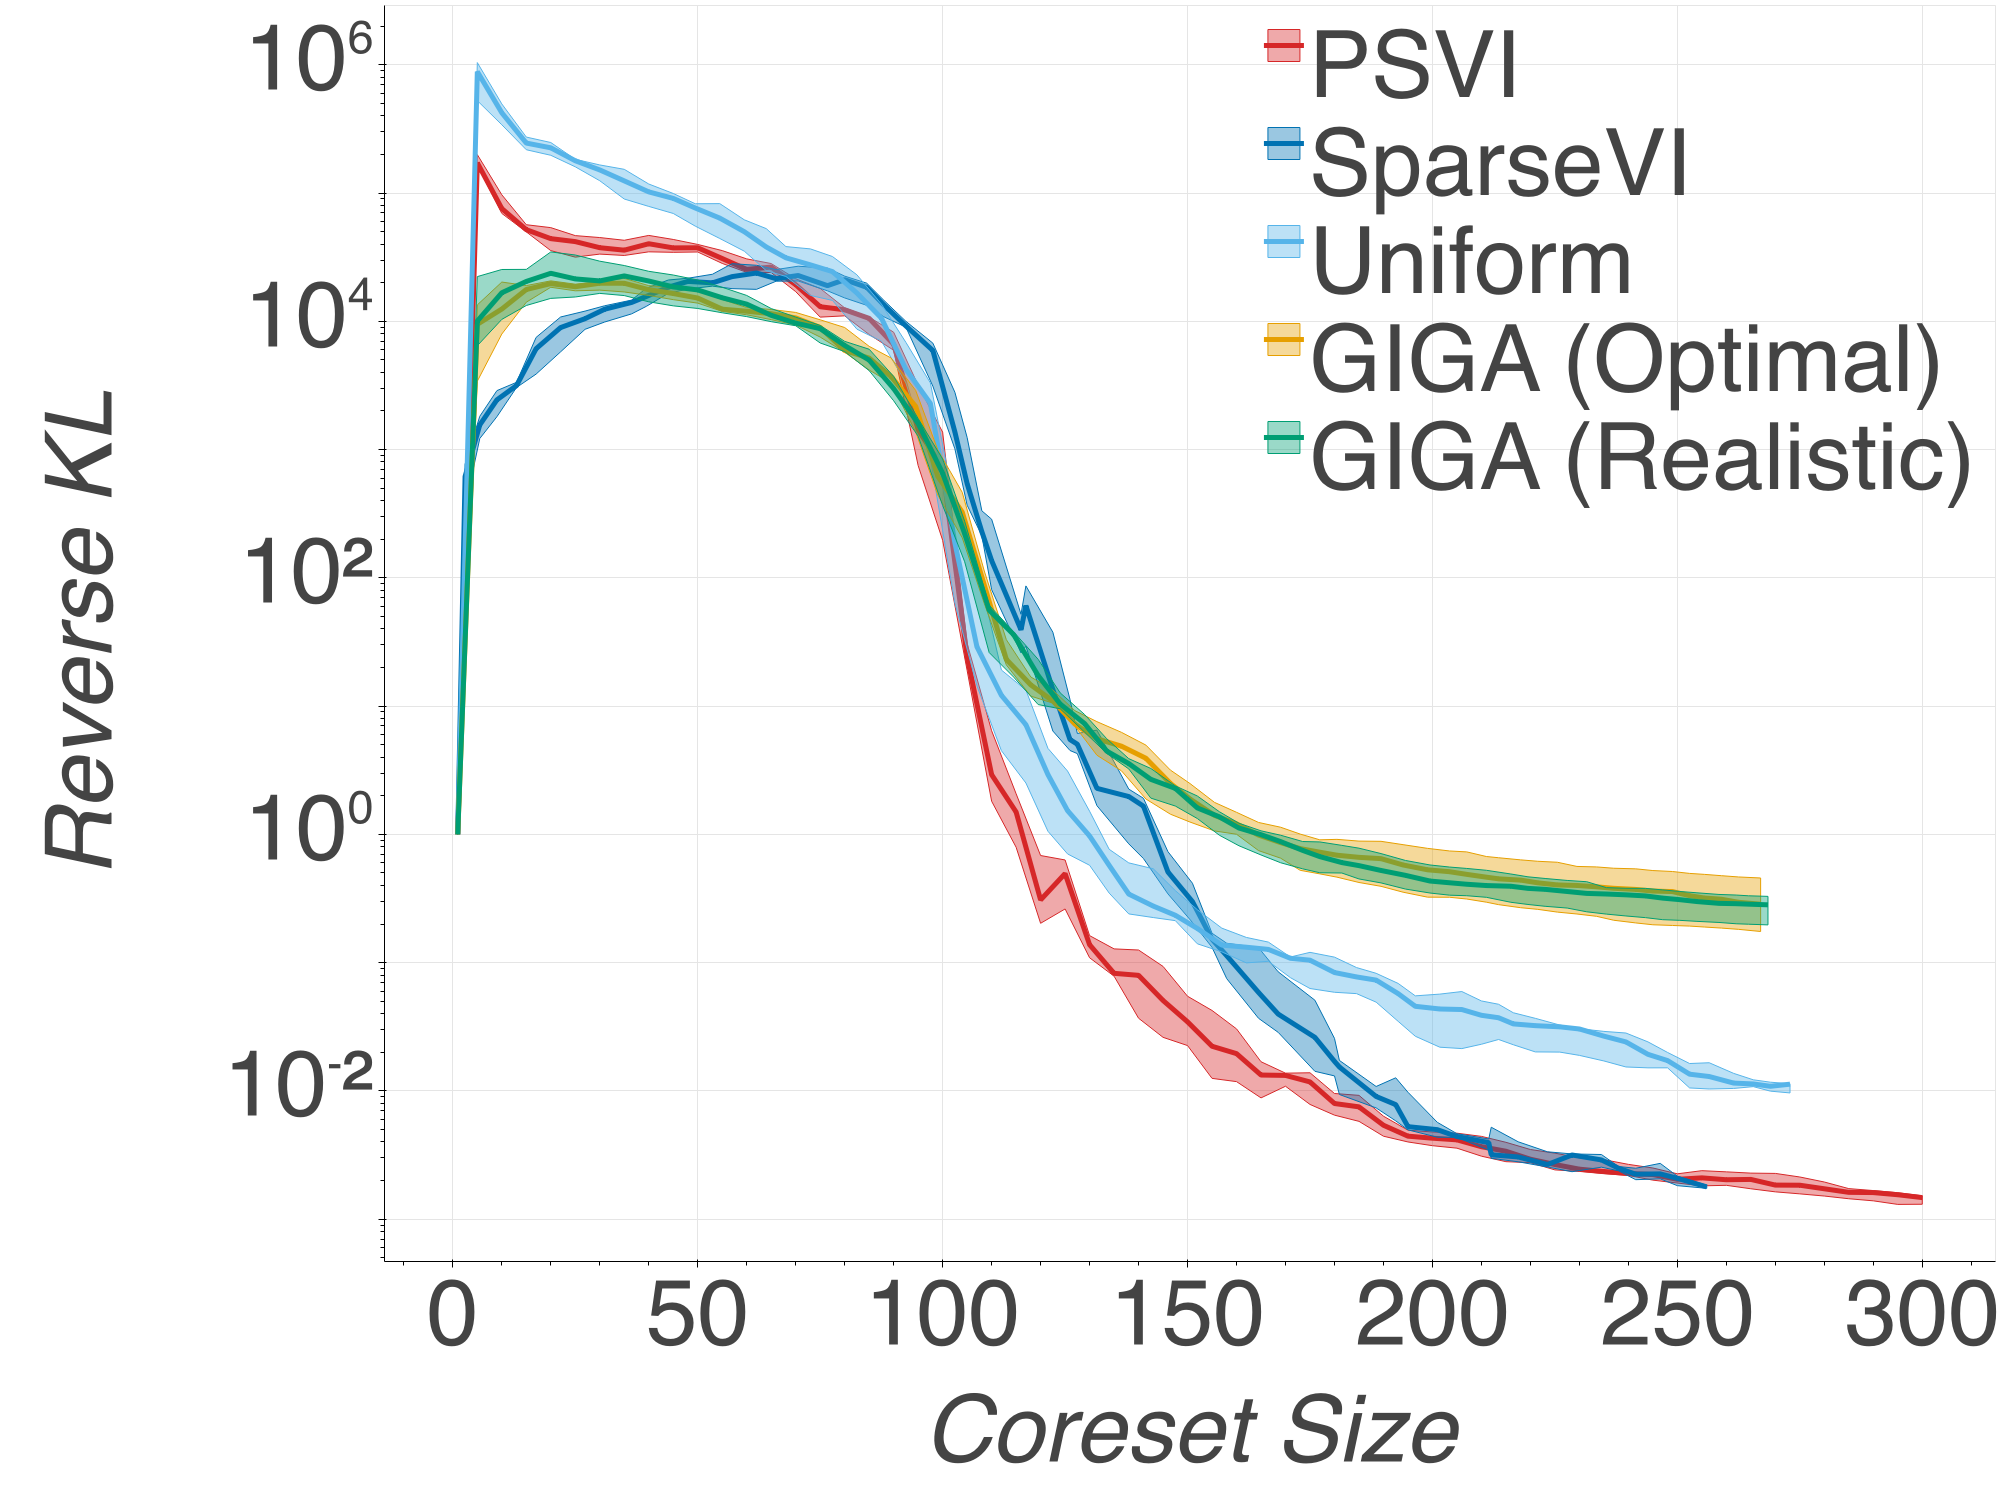
\includegraphics[width=1.15\columnwidth]{\MyPath/figs/linregKLDvsCstSize_200.png}}%
		\caption{$\text{project. dim.}=200$}
	\end{subfigure}\hfill\qquad
	\centering
	\begin{subfigure}[b]{.29\textwidth}
		\centerline{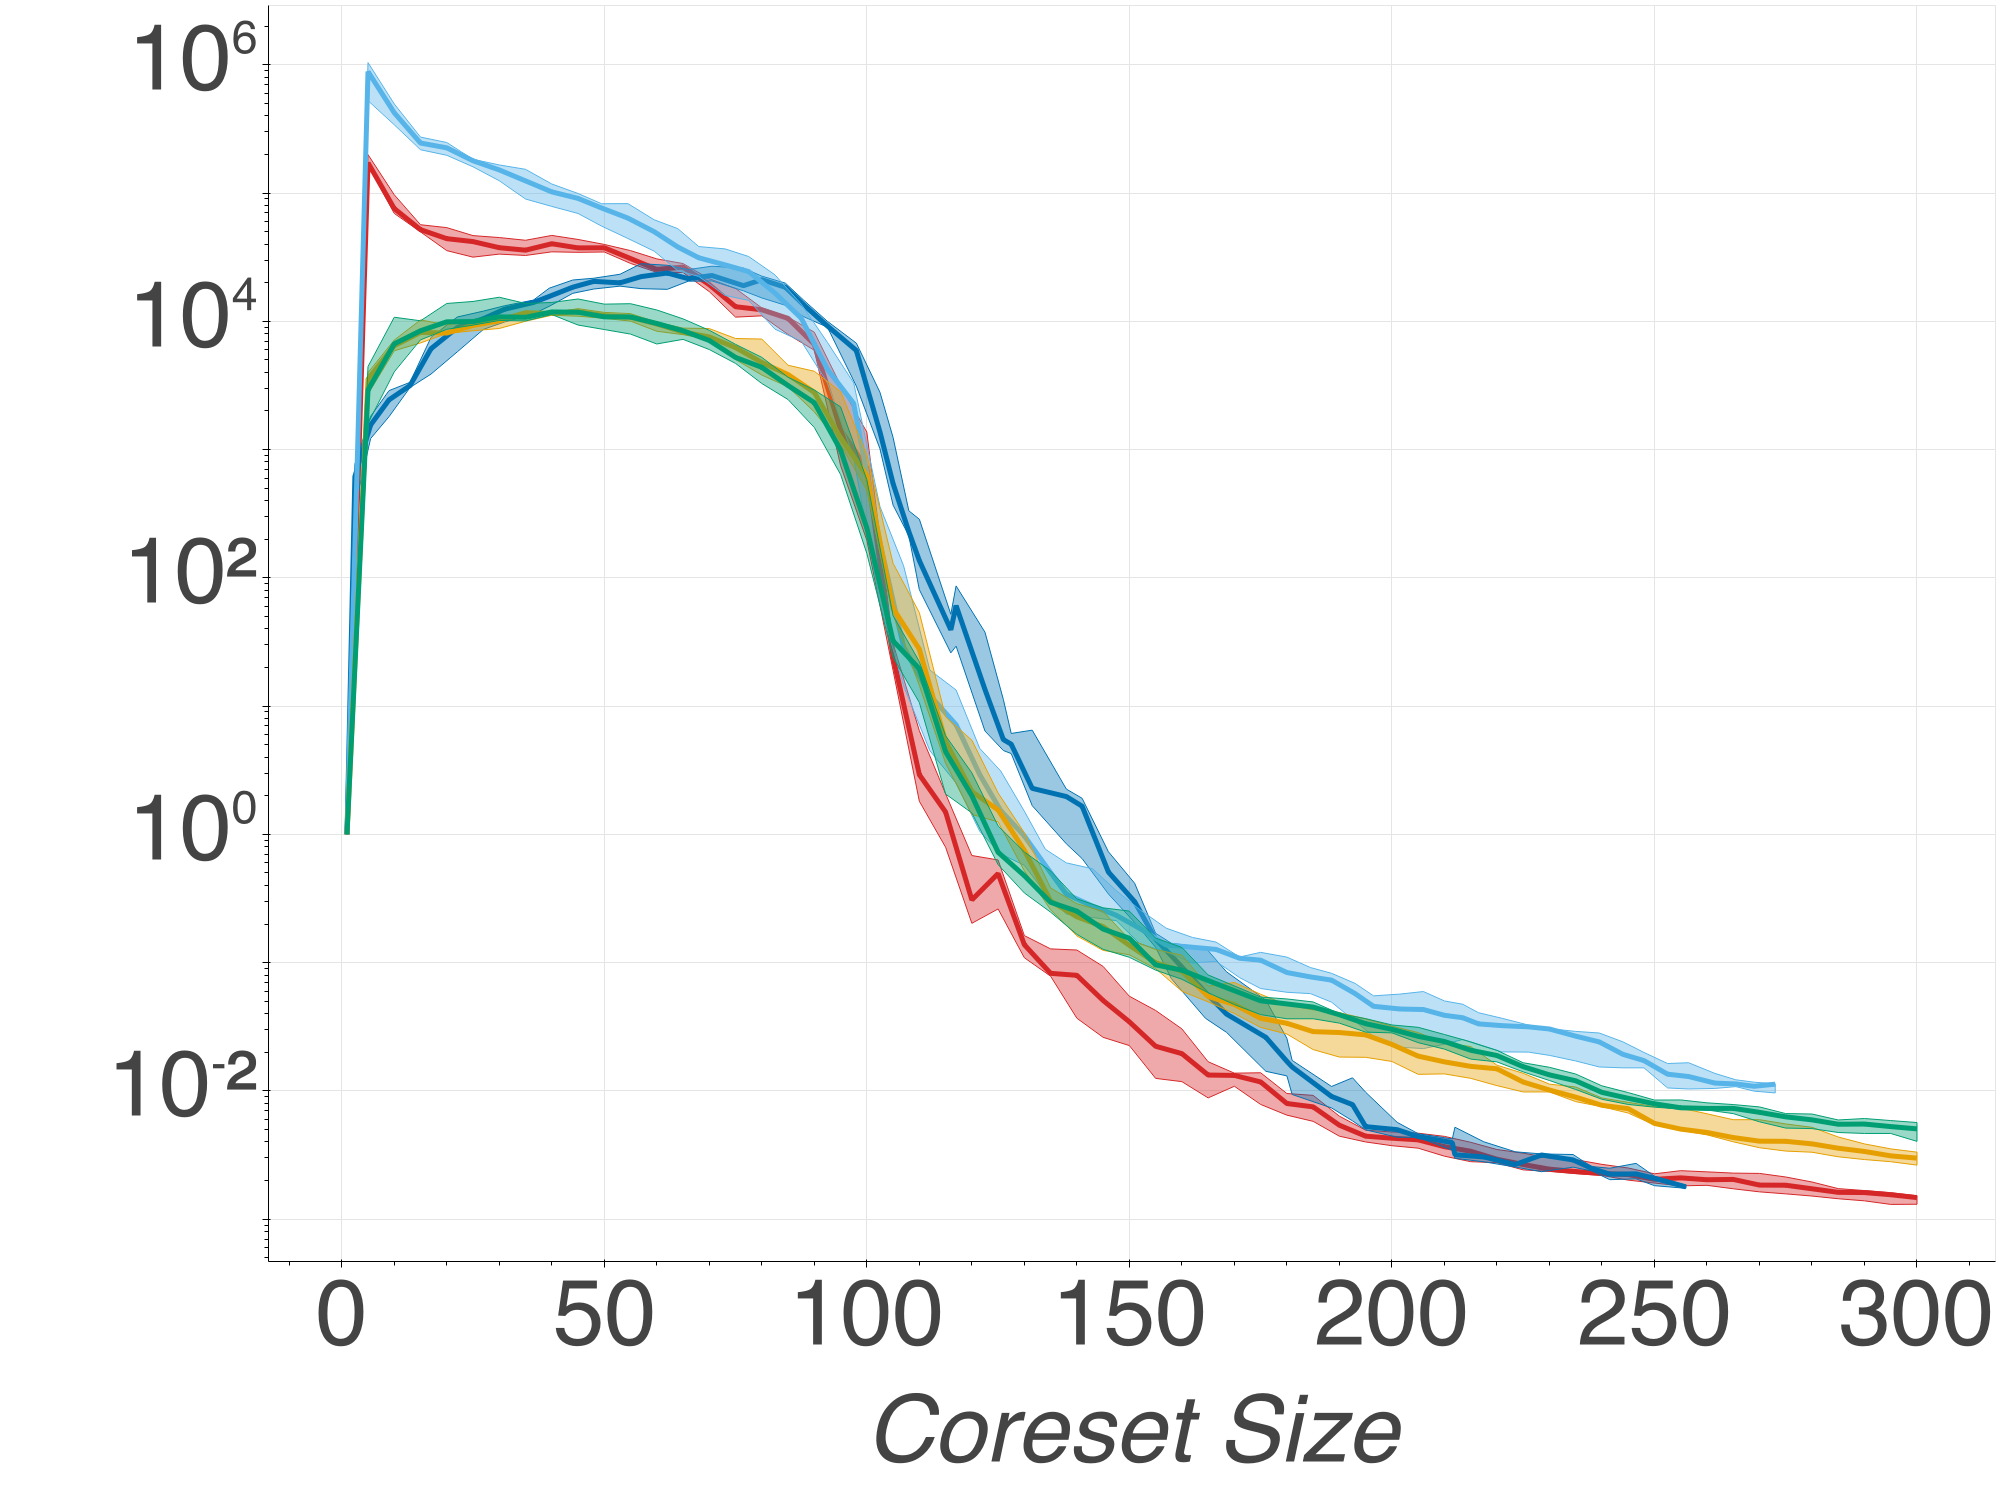
\includegraphics[width=1.15\columnwidth]{\MyPath/figs/linregKLDvsCstSize_2000.png}}%
		\caption{$\text{project. dim.}=2,000$}
	\end{subfigure}\hfill\qquad
	\centering
	\begin{subfigure}[b]{.29\textwidth}
		\centerline{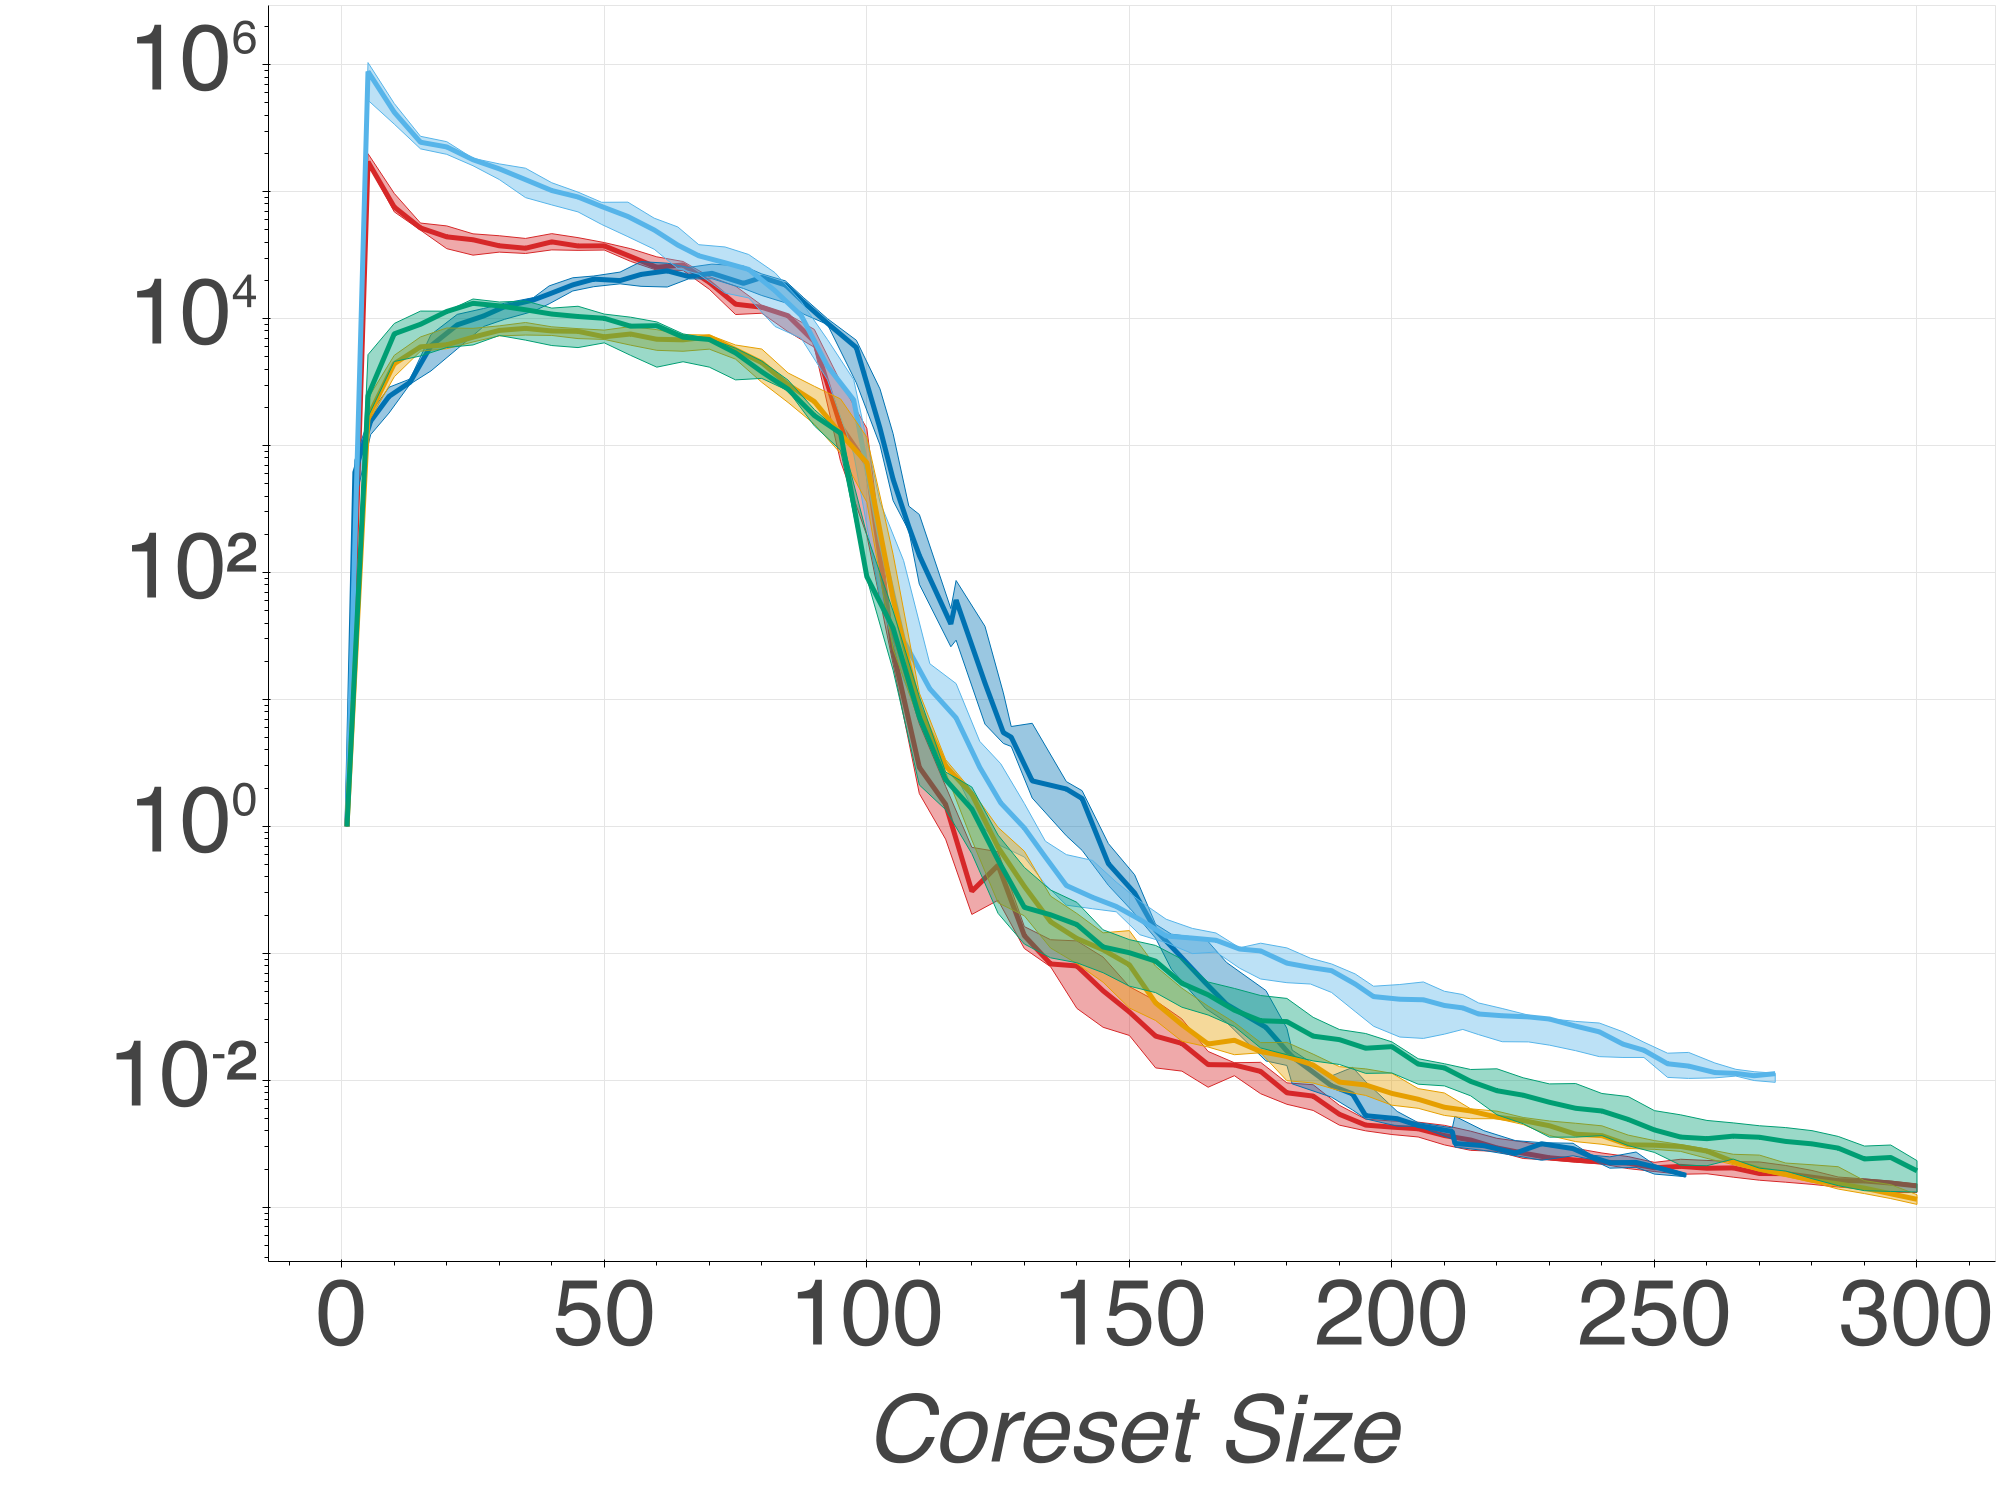
\includegraphics[width=1.15\columnwidth]{\MyPath/figs/linregKLDvsCstSize_10000.png}}%
		\caption{$\text{project. dim.}=10,000$}
	\end{subfigure}
	\caption{Comparison of Hilbert coresets performance on Bayesian linear regression experiment for increasing projection dimension (over 10 trials).}
	\label{fig:hilbert_varying_projdim}
\end{figure}

Here we present some more plots demonstating the dependence of Hilbert coresets approximation quality on the dimension of random projections in the Bayesian linear regression setting presented in~\cref{fig:linreg_300}. We remind that the dimension used at this experiment and throughout the entire experiments section was set to 100. Increasing this number is typically expensive to obtain in practice. As demonstrated in~\cref{fig:hilbert_varying_projdim}, getting higher projection dimension enables better posterior approximation in the problem for both \gigao~and~\gigar. However, \psvi~remains competitive in the small coreset regime, even for Hilbert coresets with extremely large projection dimensionality, demonstrating the information-geometric limitations that Hilbert coreset constructions are known to face~\cite{campbell19neurips}.


\subsection{Bayesian logistic regression}
\label{app:logreg_experiment_appendix}

\subsubsection{Model}
\label{app:logreg_model_appendix}
In logistic regression we have a set of datapoints $(x_n, y_n)_{n=1}^{N}$ each corresponding to a feature vector ${x_n \in \reals^d}$ and a label ${y_n \in \{-1, 1\}}$. Datapoints are assumed to be generated according to following statistical model
\[
y_n | x_n, \theta \sim \distBern \left( \frac{1}{1+e^{-z_n^T \theta}} \right) 
\quad 
z_n := \begin{bmatrix}
x_n \\
1
\end{bmatrix}.
\label{eq:logreg-model}
\]
The aim of inference is to compute the posterior over the latent parameter $ \theta = [\theta_0 \ldots \theta_d]^T \in \reals^{d+1}$.
Log-likelihood of each datapoint can be expressed as
\[
\begin{split}
f_n(x_n, y_n|\theta)  
=&\ind{[y_n=-1]}\log \left( 1 - \frac{1}{1+e^{-z_n^T \theta}}\right) 
- \ind{[y_n=1]} \log \left( 1+ e^{-z_n^T \theta}  \right) \\
=&-\log\left( 1 + \exp(-y_n z_n^T\theta)\right).
\label{eq:logreg-loglik}
\end{split}
\]
Hence in pseudocoreset construction we can optimize pseudodata point locations with respect to continuous variable $ x_n$, using the gradient
\[
\nabla_{x_n}f_n =  \frac{e^{-y_n z_n^T \theta}}{1+e^{-y_n z_n^T \theta}}y_n \begin{bmatrix}
\theta_1 \\
\vdots \\
\theta_d
\end{bmatrix}.
\label{eq:logreg-loglik-locgrad}
\]



\subsubsection{Datasets description}
\label{app:logreg_data_details}
For logistic regression experiments, we used subsampled and full versions of datasets presented in~\cref{table:datasets_details}: a synthetic dataset with $ x\in \reals^2 $ sampled \iid from a $\distNorm{(0, I)}$ and $ y\in\{-1,1\} $ sampled from respective logistic likelihood with $ \theta =[3, 3, 0]^T$ (\textsc{Synthetic}); a phishing websites dataset reduced to $ D=10 $ via PCA (\textsc{Phishing}); a chemical reactivity dataset with  real-valued features corresponding to its first $ 10 $ and $ 100 $ principal components (\textsc{ChemReact} and \textsc{ChemReact100} respectively); a dataset with $ 50 $ real-valued features associated with whether each of $ 100K $ customers of a bank will make a specific transaction (\textsc{Transactions}); and a dataset for music analysis, where we consider \emph{"classical vs all"} genre classification task (\textsc{Music}). Original versions of the four latter datasets are available online respectively at~\href{https://www.csie.ntu.edu.tw/~cjlin/libsvmtools/datasets/binary.html}{https://www.csie.ntu.edu.tw/\~{}cjlin/libsvm tools/datasets/binary.html},  \href{http://komarix.org/ac/ds/}{http://komarix.org/ac/ds},  \href{https://www.kaggle.com/c/santander-customer-transaction-prediction/data}{https://www.kaggle.com/c/santan der-customer-transaction-prediction/data}, and \href{https://github.com/mdeff/fma}{https://github.com/mdeff/fma}. 

\begin{table}[!t]
	\begin{center}
		\begin{tabular}{|l|l|l|}
			\hline
			\textbf{Dataset name}       & $N$      & $D$   \\ \hline
			\textsc{Synthetic}  & 500    & 2   \\ \hline
			\textsc{Phishing}   & 500    & 10  \\ \hline
			\textsc{ChemReact}        & 500    & 10  \\ \hline
			\textsc{Transactions}  & 100,000   & 50   \\ \hline
			\textsc{ChemReact100}    & 26,733 & 100 \\ \hline
			%mnist      & 10,000    & 758 \\ \hline
			\textsc{Music}      & 8,419    & 237 \\ \hline
		\end{tabular}
	\end{center}
	\caption{Details for datasets used in logistic regression experiments.}
	\label{table:datasets_details}
\end{table}

\subsubsection{Small-scale experiments}
\label{app:small_scale_appendix}
In the small-scale experiment, the number of overall gradient updates was
set to $T = 1,500$, while minibatch size was set to  $B = 400$. Learning rate schedule for \sparsevi~and \psvi~was ${\gamma_t = 0.1t^{-1}}$. Results presented in~\cref{fig:smallscale_ls_blogreg_dkl} indicate that~\psvi~achieves superior quality to~\sparsevi~for small coreset sizes, and is competitive to~\gigao, while the latter unrealistically uses true posterior samples to tune a weighting function required over construction.


\begin{figure*}[!t]
	\centering
	\begin{subfigure}[b]{.29\textwidth}
		\caption*{\textsc{Synthetic}}
		\vspace*{-0.3cm}
		\centerline{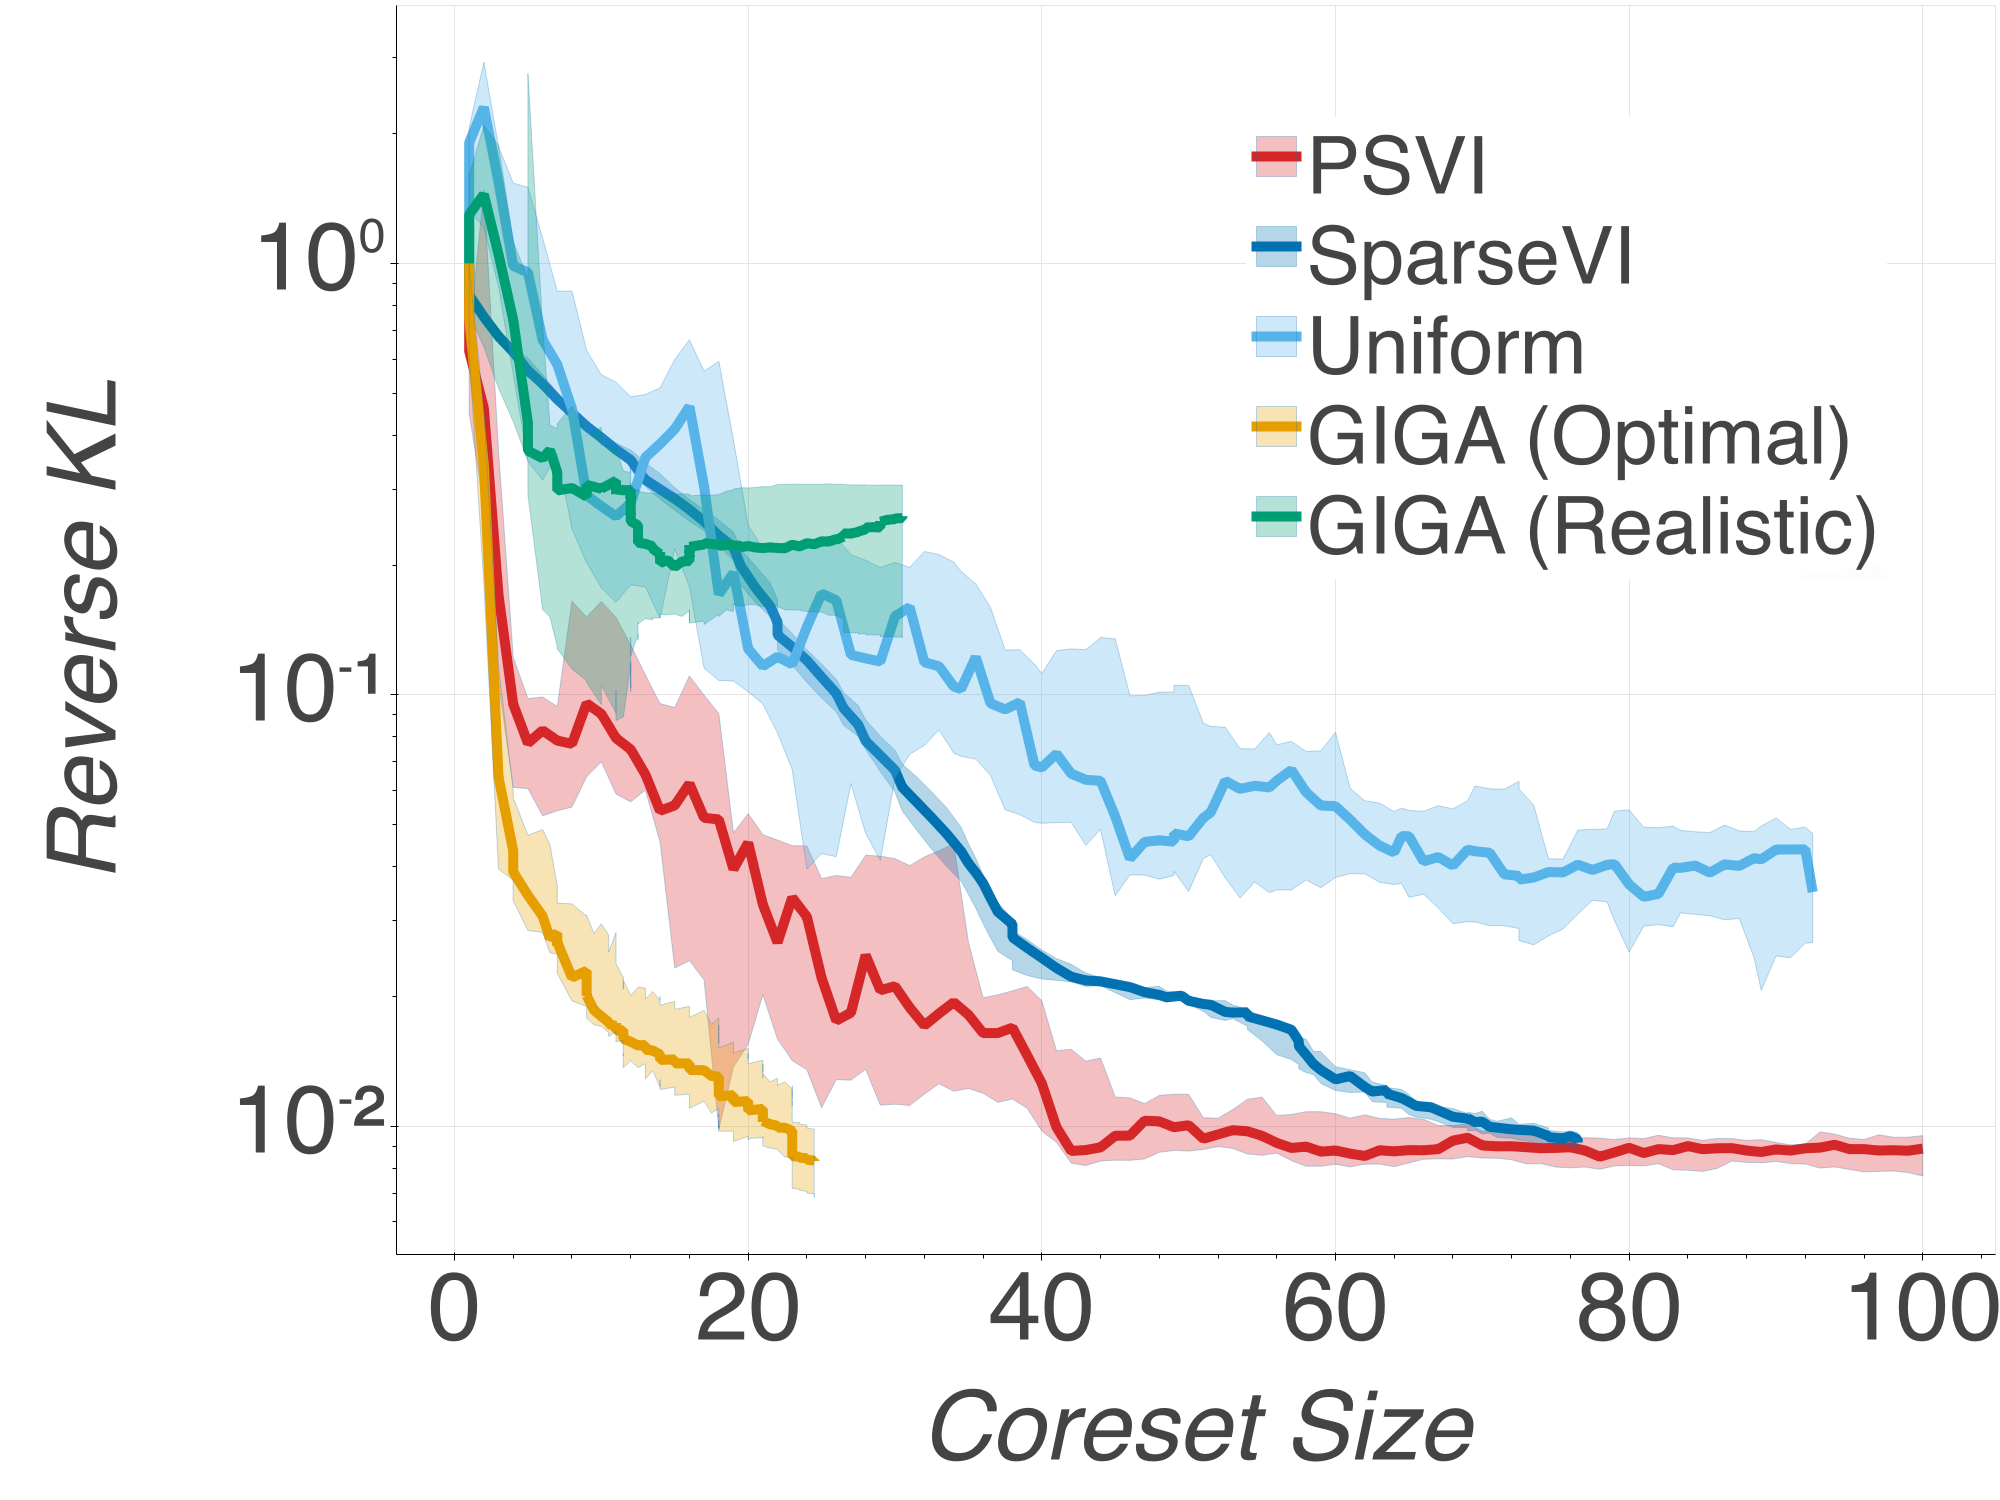
\includegraphics[width=1.15\columnwidth]{\MyPath/figs/synth_lr_KLDvssz.png}}%
	\end{subfigure}\hfill\qquad
	\centering
	\begin{subfigure}[b]{.29\textwidth}
		\caption*{\textsc{Phishing}}
		\vspace*{-0.3cm}
		\centerline{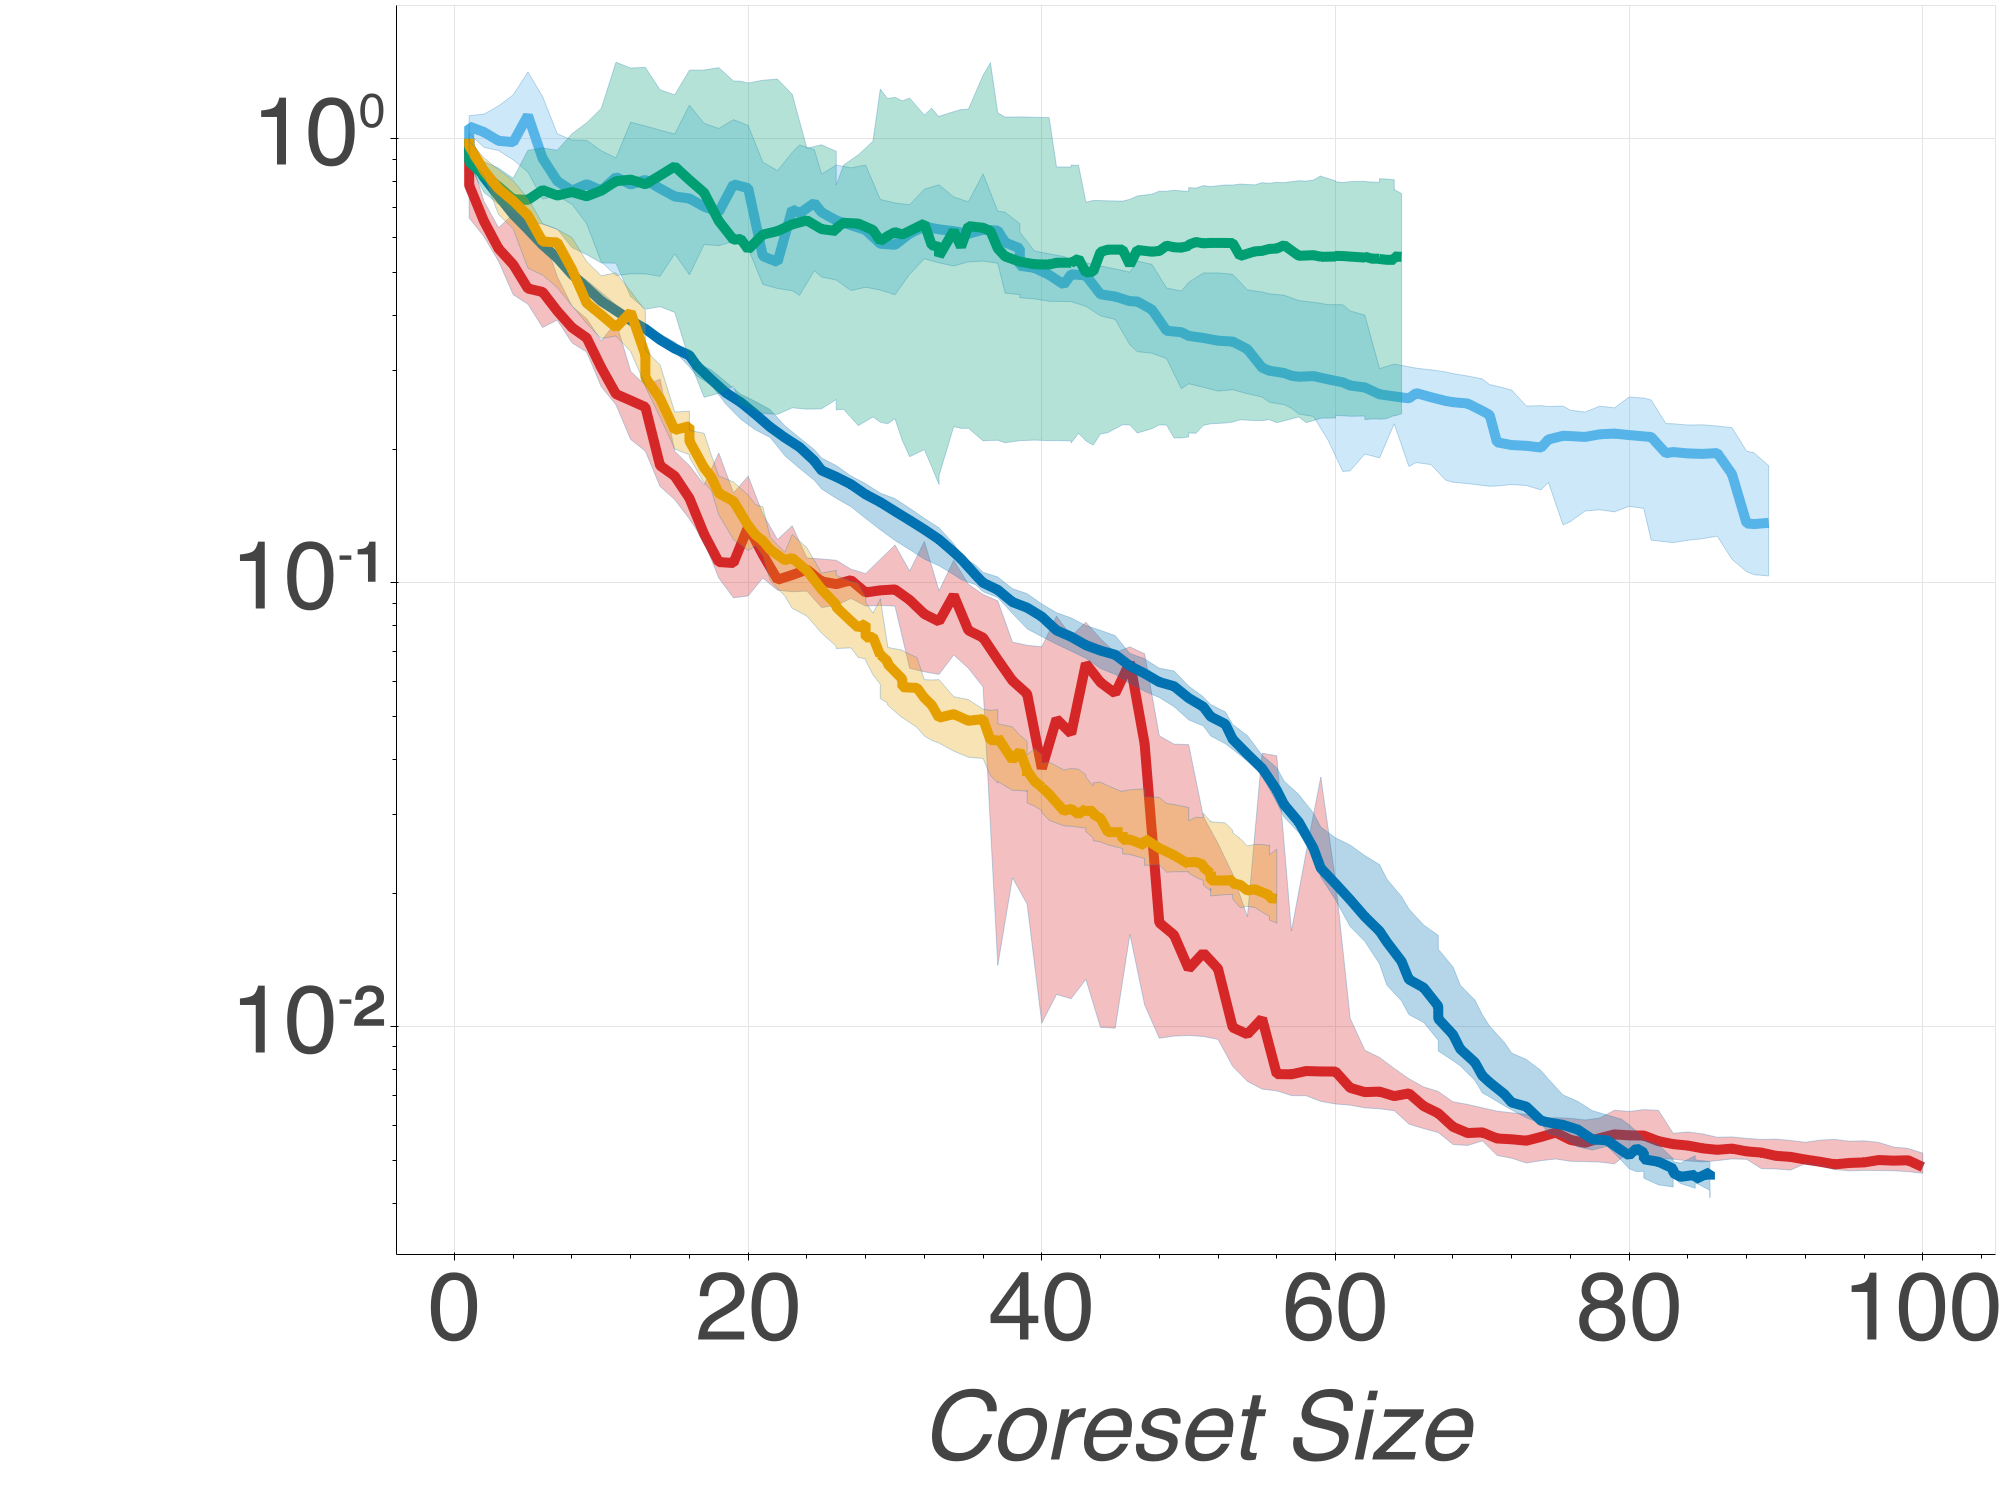
\includegraphics[width=1.15\columnwidth]{\MyPath/figs/phishing_KLDvssz.png}}%
	\end{subfigure}\hfill\qquad
	\centering
	\begin{subfigure}[b]{.29\textwidth}
		\caption*{\textsc{ChemReact}}
		\vspace*{-0.3cm}
		\centerline{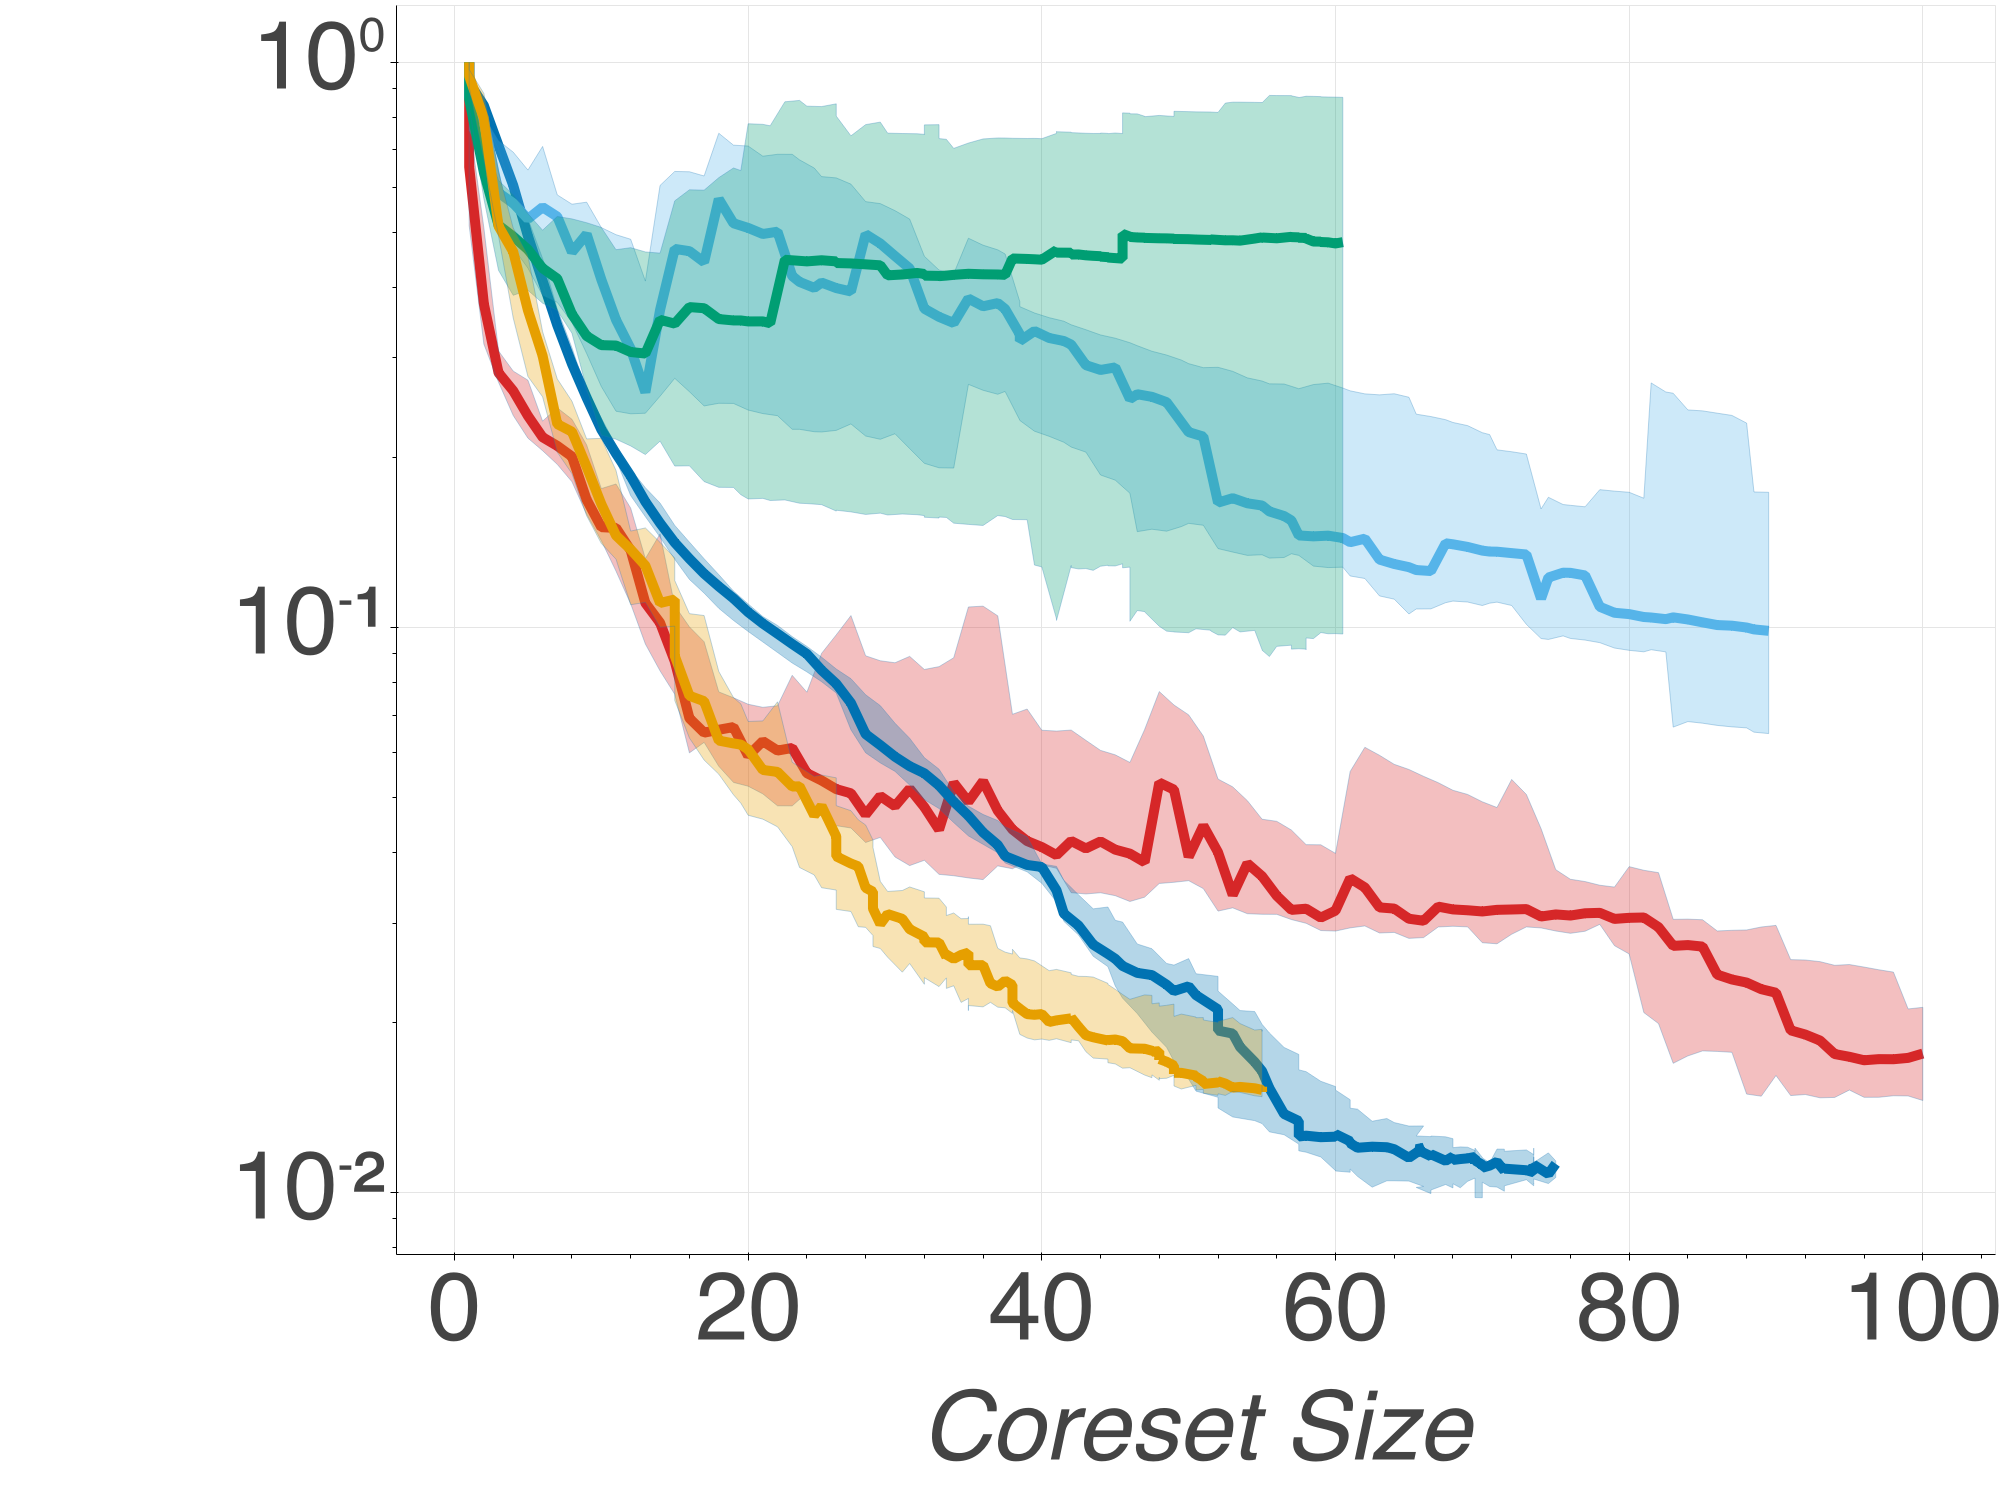
\includegraphics[width=1.15\columnwidth]{\MyPath/figs/ds1_KLDvssz.png}}%
	\end{subfigure}
	\caption{Comparison of (pseudo)coreset approximate posterior
		quality vs  coreset
		size for logistic regression over 10 trials.}
	\label{fig:smallscale_ls_blogreg_dkl}
\end{figure*}

\subsubsection{Reproducibility of Bayesian logistic regression experiment}
\label{app:reproducibility}
In this subsection we provide additional details for reproducibility of the experimental setup for the Bayesian Logistic Regression experiment presented in~\cref{sec:experiments}.  

\paragraph{Posterior approximation metrics, coreset gradients and learning rates} Posterior approximation quality was estimated via computing KL divergence between Gaussian distributions fitted on coreset and full data posteriors via Laplace approximation. For both \sparsevi~and \psvi, gradients were estimated using samples drawn from a Laplace approximation fitted on current coreset weights
and points. To optimize initial learning rates for \sparsevi~and \psvi, we did a grid search over ${\{0.1, 1, 10\}}$.

\paragraph{Differential privacy loss accounting and hyperparameter selection}  In the differential privacy experiment, we were not concerned with the extra privacy cost of hyperparameter optimization task.  Estimation of differential privacy cost at all experiments was based on TensorFlow privacy implementation of moments accountant for the subsampled Gaussian mechanism.\footnote{\href{https://github.com/tensorflow/privacy}{https://github.com/tensorflow/privacy}} 
For \dpsvi~we used the best learning hyperparameters found for \psvi~on the corresponding dataset. The demonstrated range of privacy budgets was generated by decreasing the variance $ \sigma $ of additive Gaussian noise and keeping the rest of hyperparameters involved in privacy accounting fixed.  
Regarding \dpvi, over our experiments we also kept subsampling ratio fixed. We based our implementation of \dpvi~on authors code,\footnote{\href{https://github.com/DPBayes/DPVI-code}{https://github.com/DPBayes/DPVI-code}} adapting noise calibration according to the adjacency relation used in~\cref{sec:dp-pseudocoresets}, and the standard differential privacy definition~\citep{dwork14}. In our experiment, we used the AdaGrad optimizer~\citep{duchi11}, with learning rate $0.01$, number of iterations $2,000$, and minibatch size $200$. Gradient clipping values for \dpvi~results presented in~\cref{fig:dklvseps}, for \textsc{Transactions}, \textsc{ChemReact100}, and \textsc{Music} datasets were tuned via grid search over ${\{1, 5, 10, 50\}}$. The values of gradient clipping constant giving best privacy profiles for each dataset, used in~\cref{fig:dklvseps}, were 10, 5, and 5 respectively. 



\subsubsection{Additional plots}
\label{app:cpu_timings}

\begin{figure*}[!t]
	\centering
	\begin{subfigure}[b]{.29\textwidth}
		\caption*{\textsc{Synthetic}}
		\vspace*{-0.3cm}
		\centerline{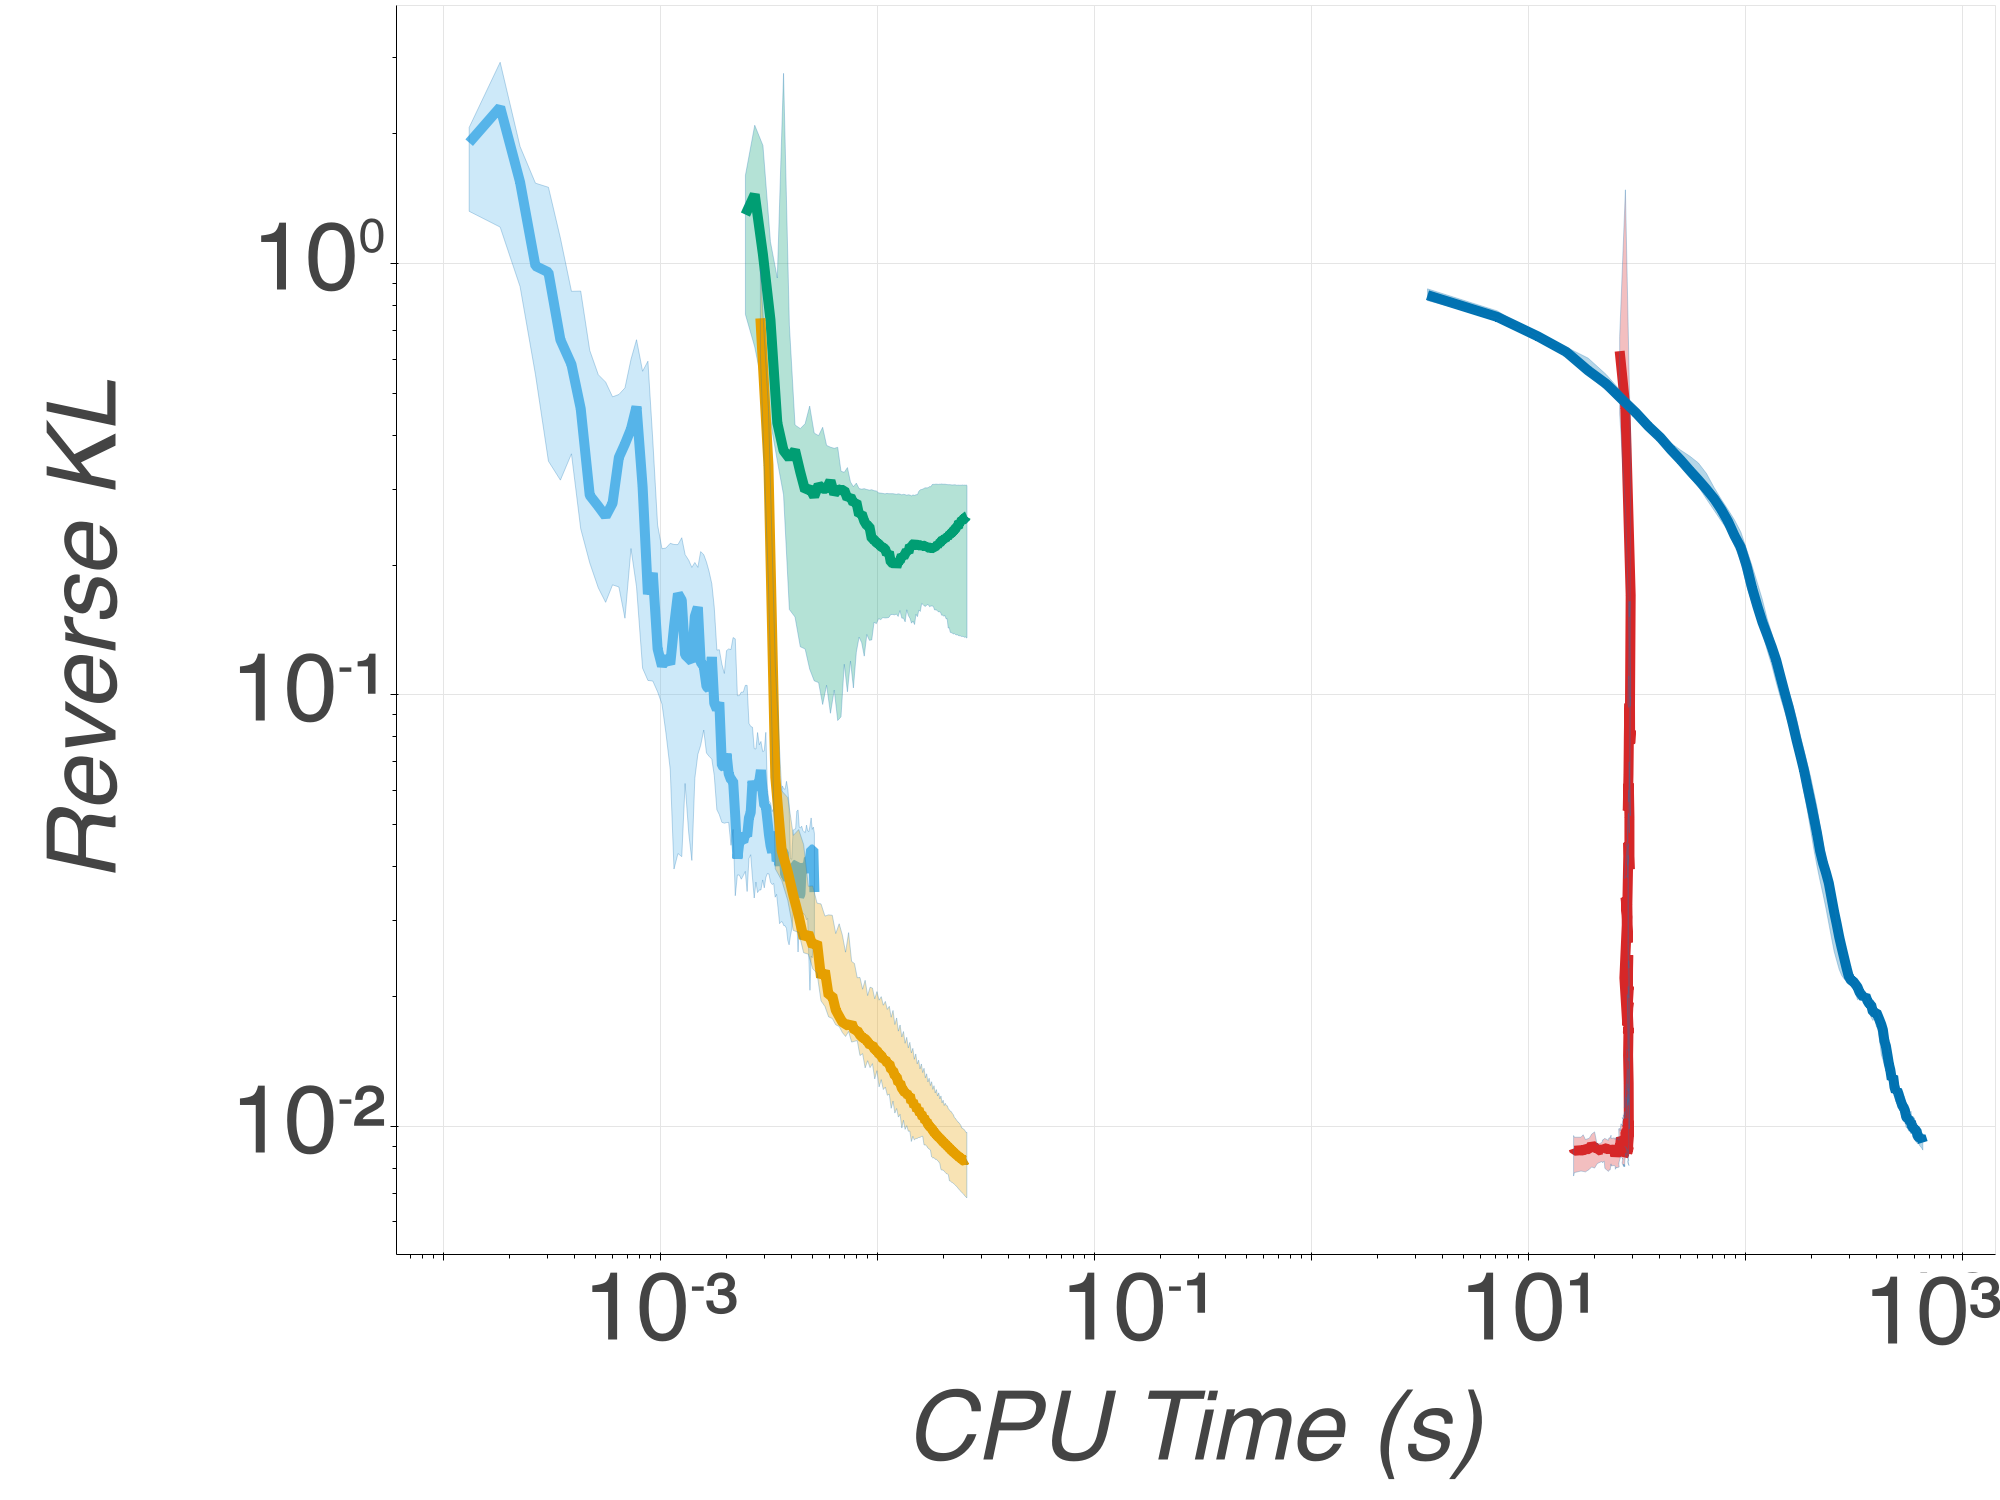
\includegraphics[width=1.15\columnwidth]{\MyPath/figs/synth_lr_KLDvscput.png}}%
	\end{subfigure}\hfill\qquad
	\centering
	\begin{subfigure}[b]{.29\textwidth}
		\caption*{\textsc{Phishing}}
		\vspace*{-0.3cm}
		\centerline{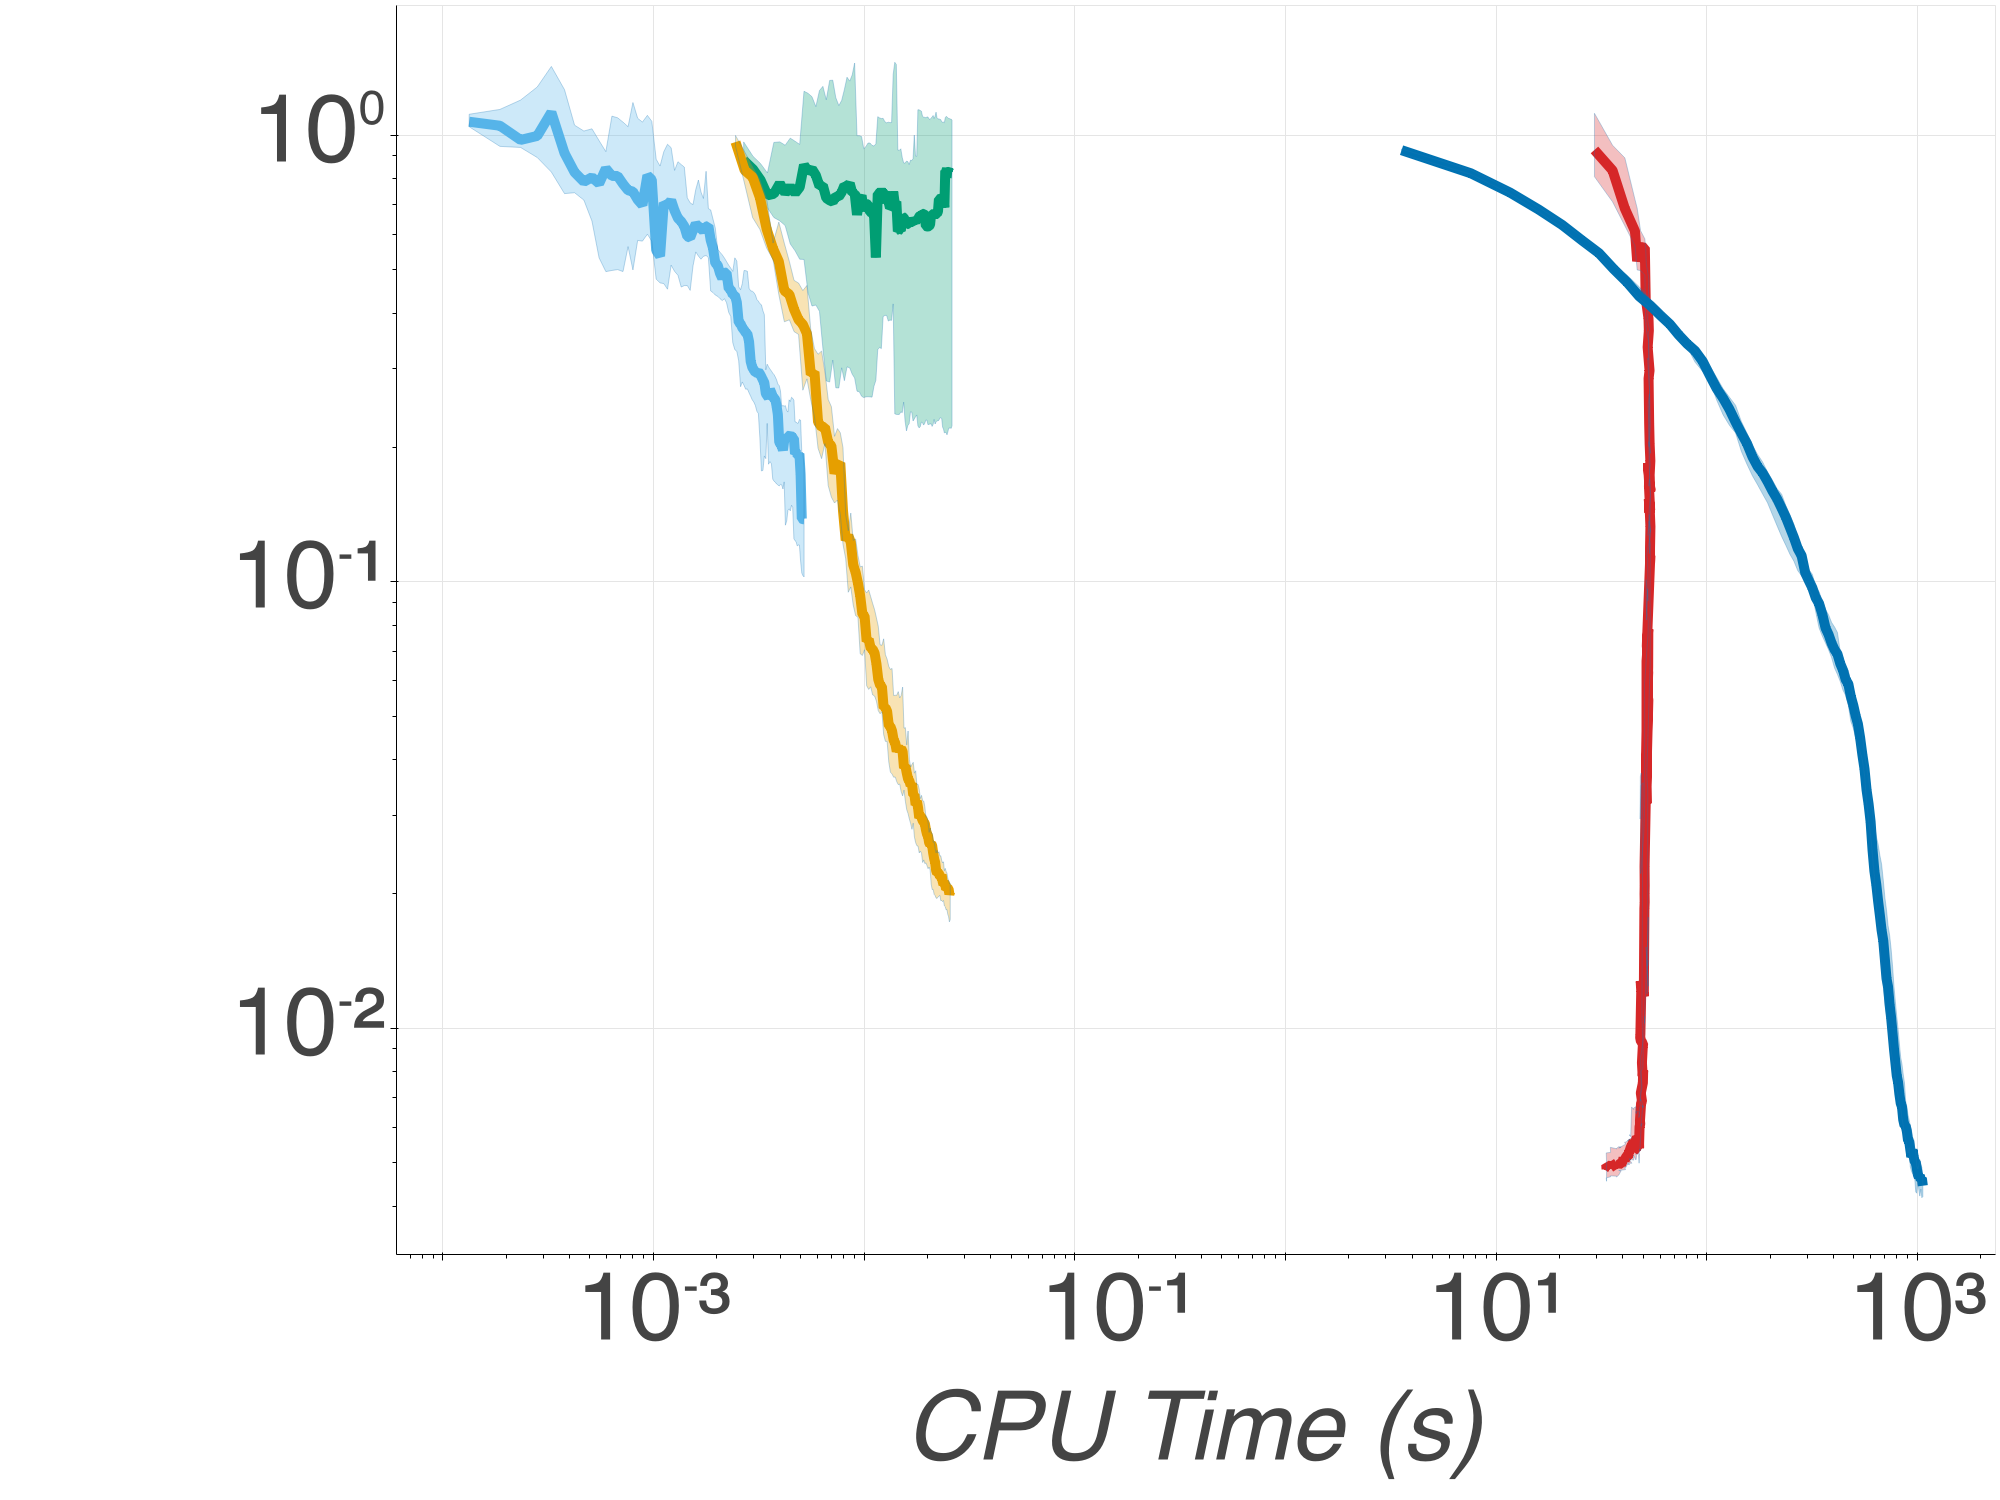
\includegraphics[width=1.15\columnwidth]{\MyPath/figs/phishing_KLDvscput.png}}%
	\end{subfigure}\hfill\qquad
	\centering
	\begin{subfigure}[b]{.29\textwidth}
		\caption*{\textsc{ChemReact}}
		\vspace*{-0.3cm}
		\centerline{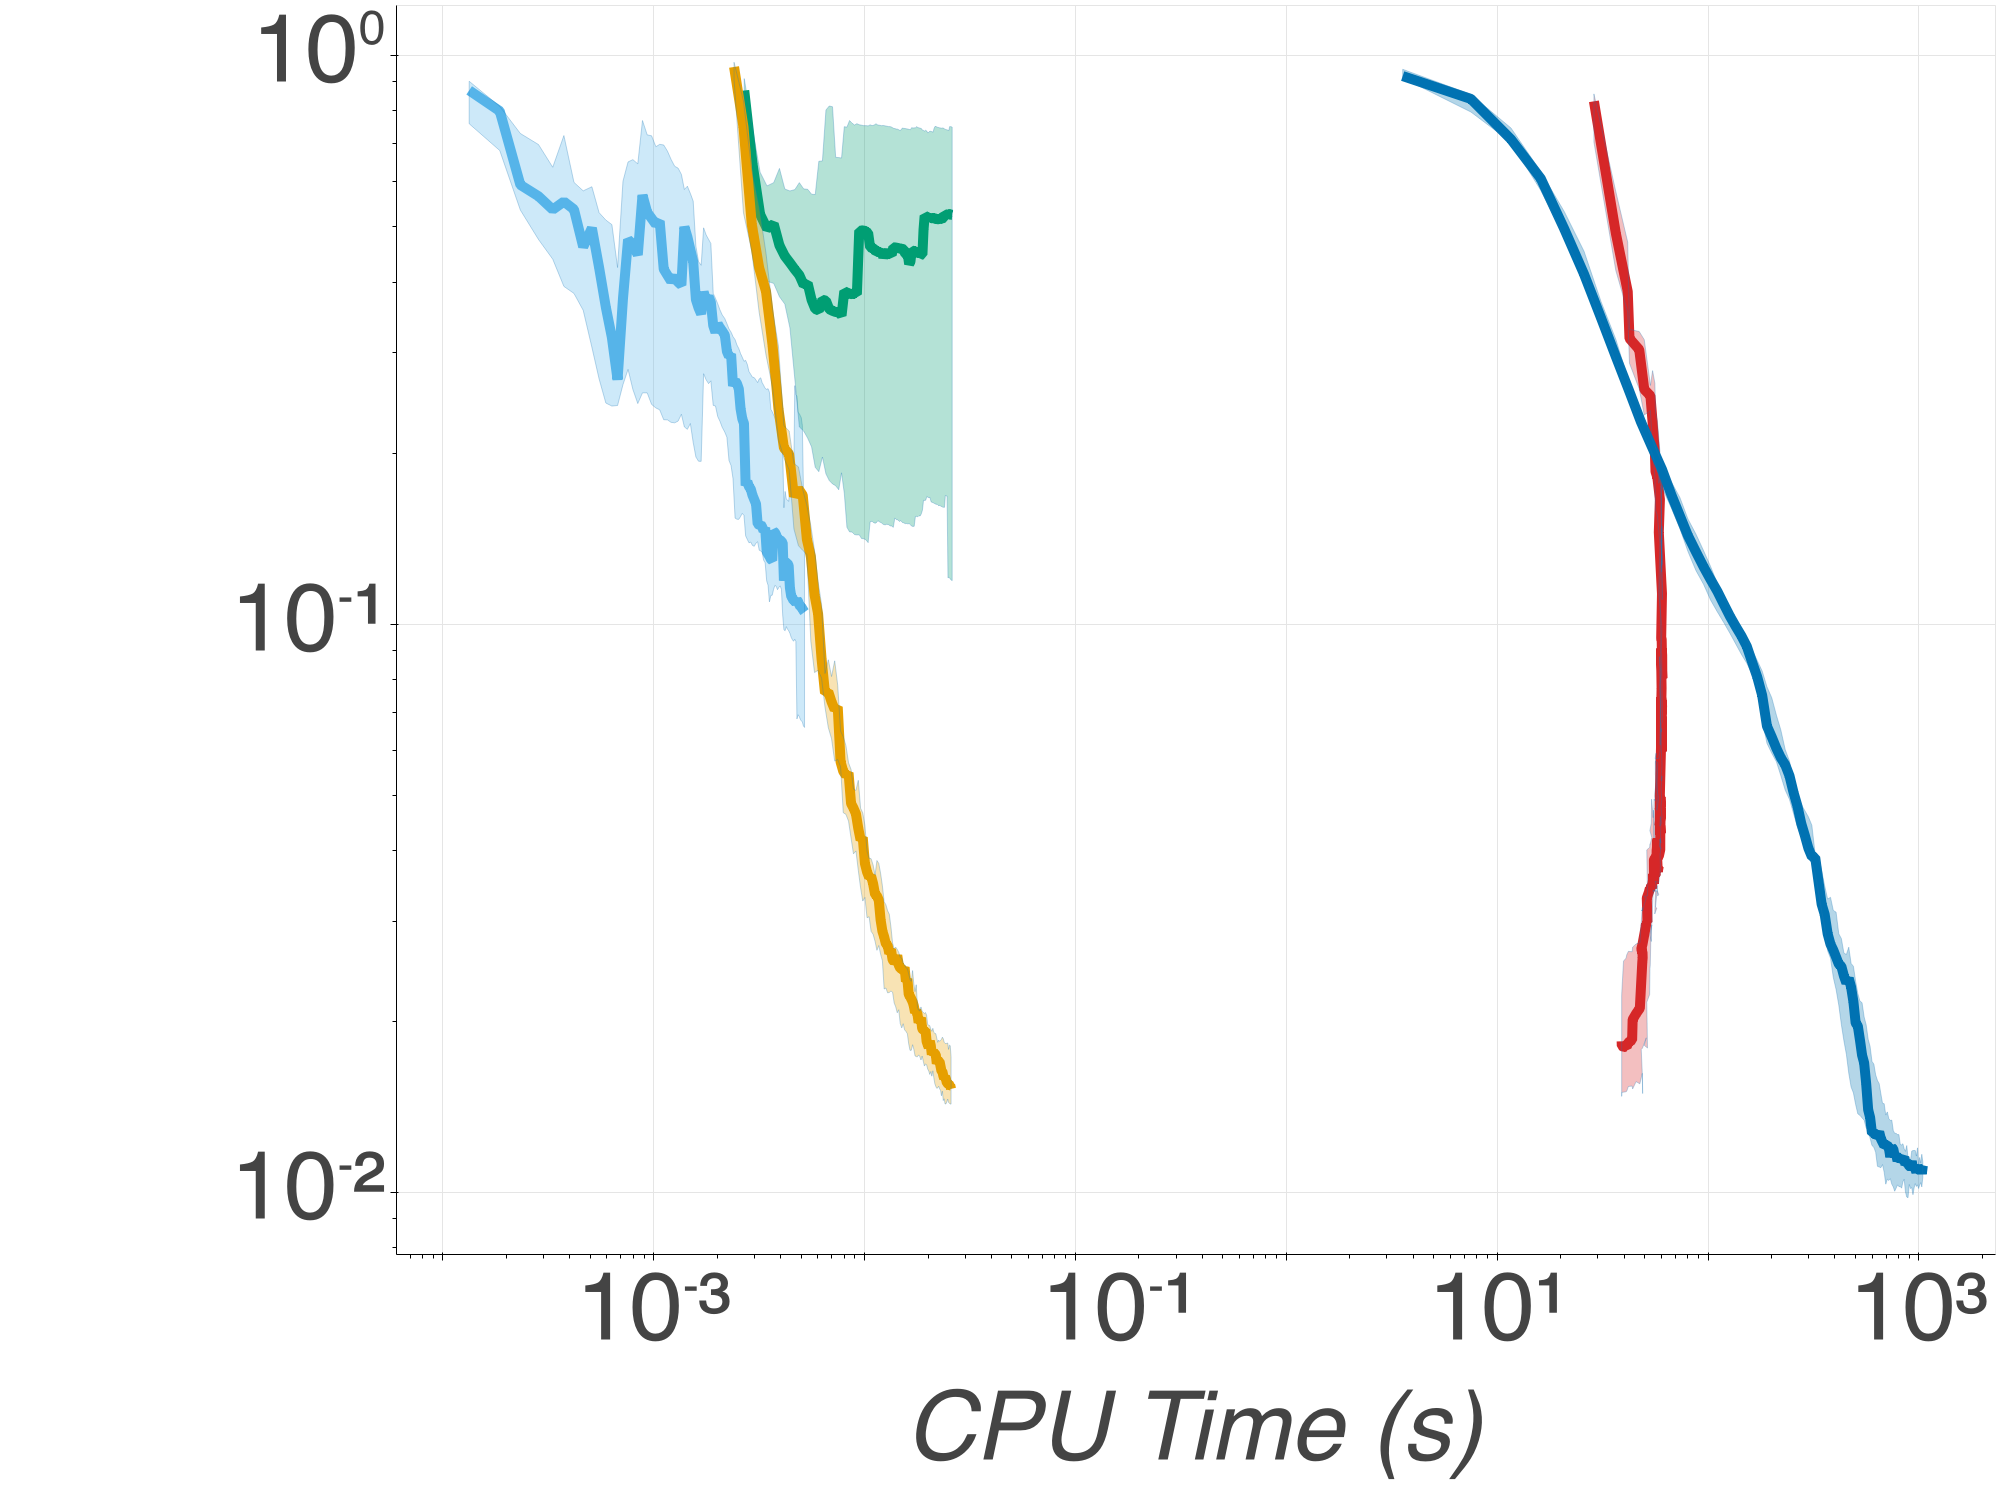
\includegraphics[width=1.15\columnwidth]{\MyPath/figs/ds1_KLDvscput.png}}%
	\end{subfigure}\hfill\qquad
	\centering
	\begin{subfigure}[b]{.29\textwidth}
		\caption*{\textsc{Transactions}}
		\vspace*{-0.3cm}
		\centerline{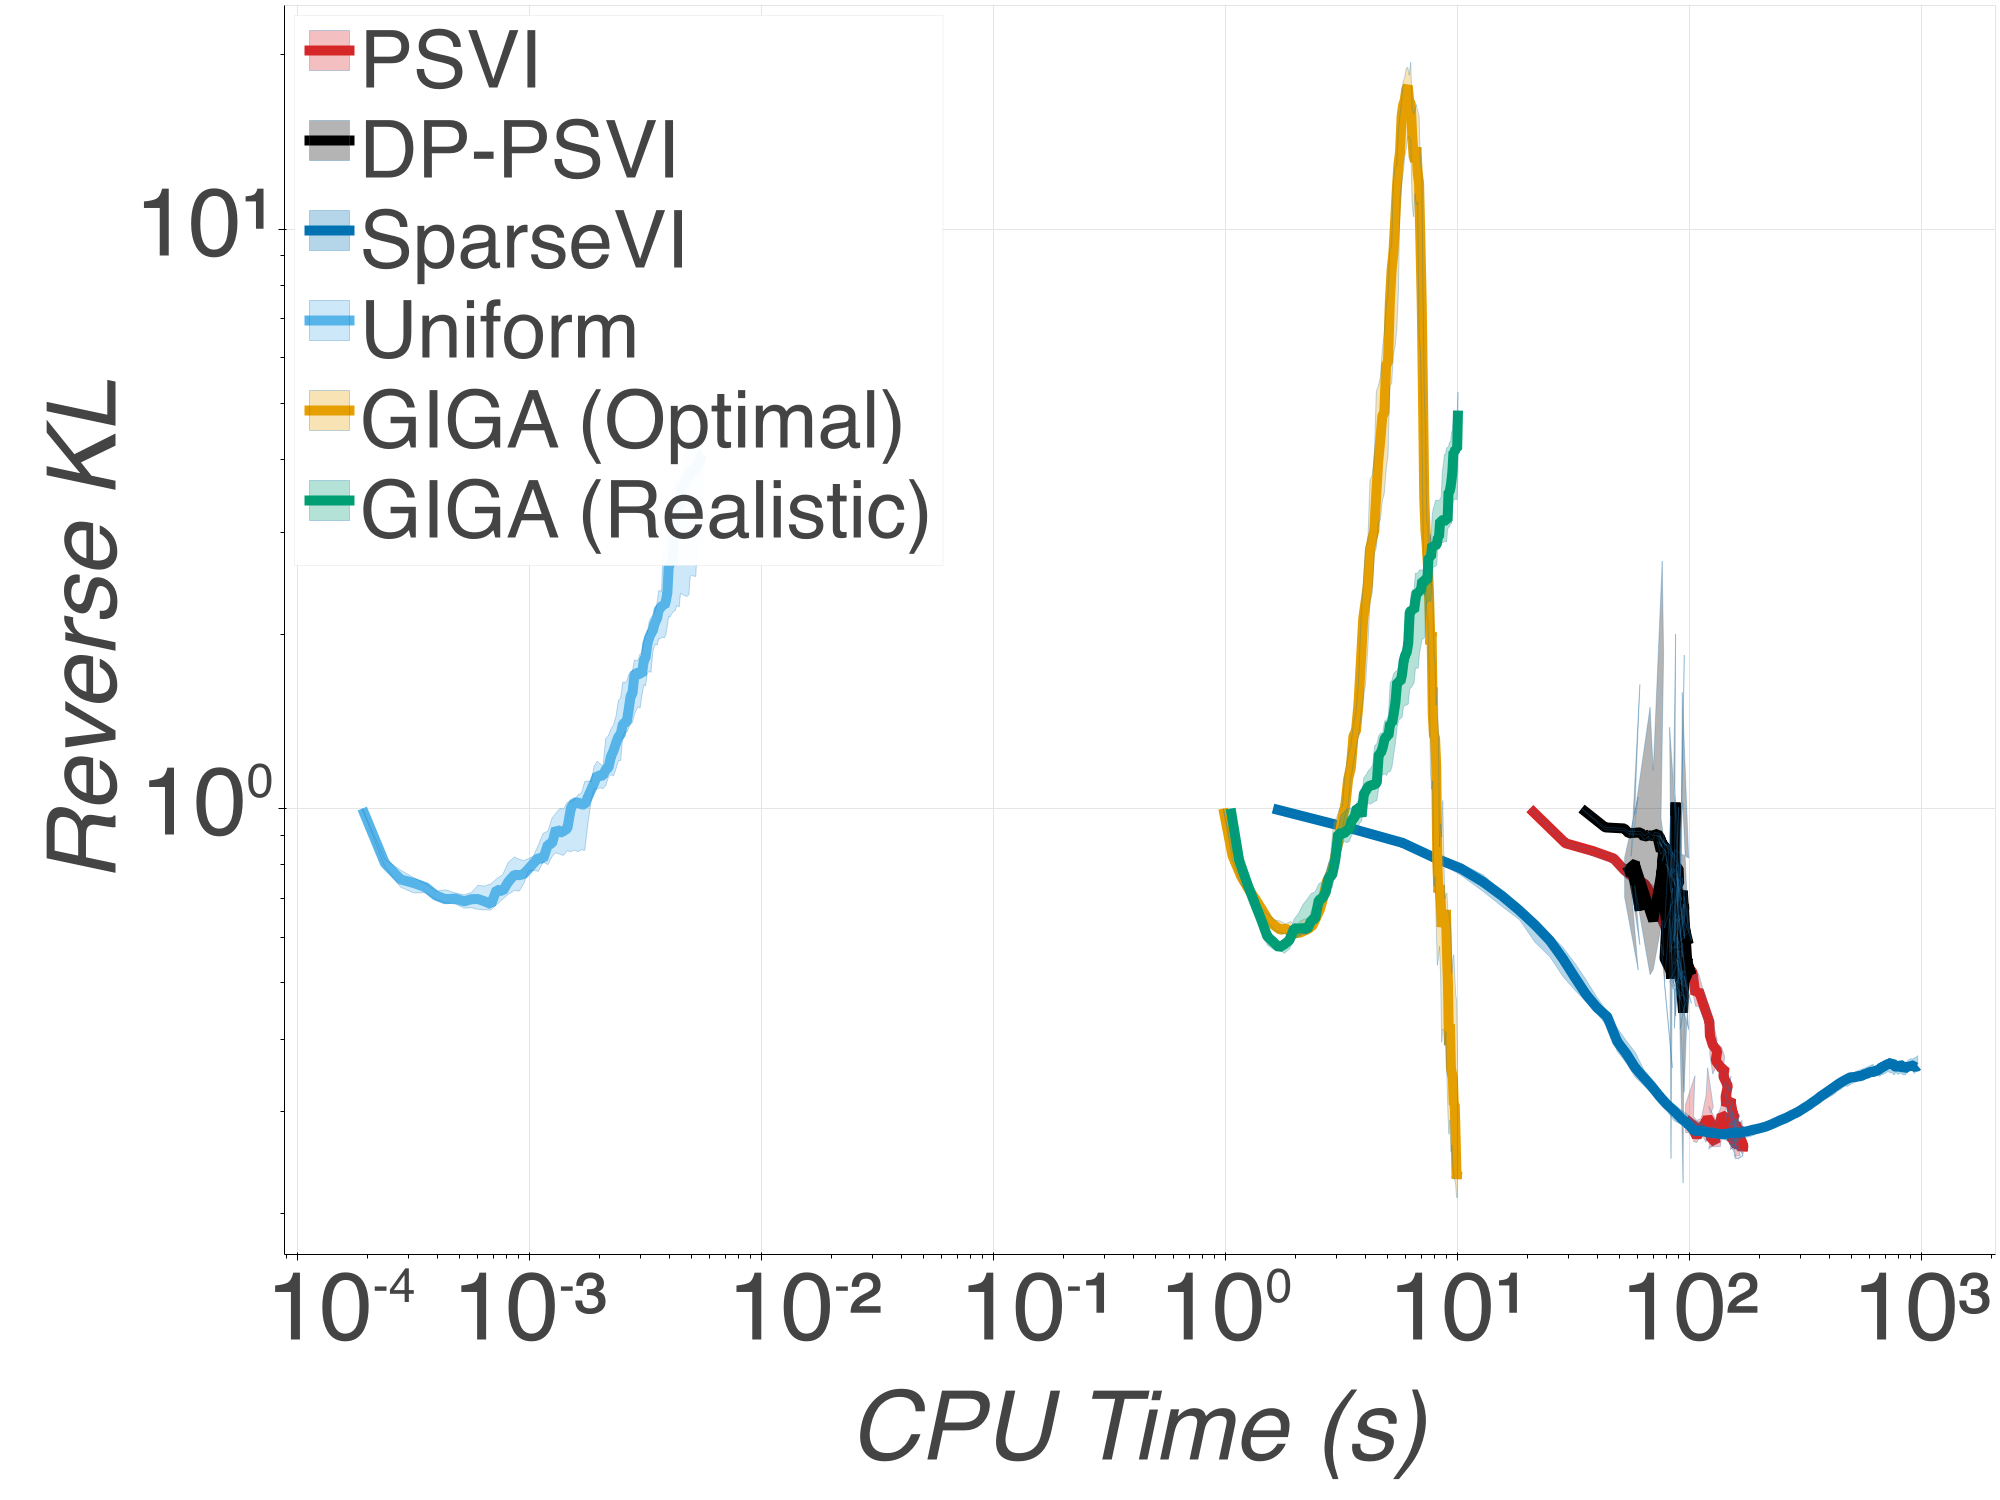
\includegraphics[width=1.15\columnwidth]{\MyPath/figs/wsanta100K_KLDvscput.png}}%
	\end{subfigure}\hfill\qquad
	\centering
	\begin{subfigure}[b]{.29\textwidth}
		\caption*{\textsc{ChemReact100}}
		\vspace*{-0.3cm}
		\centerline{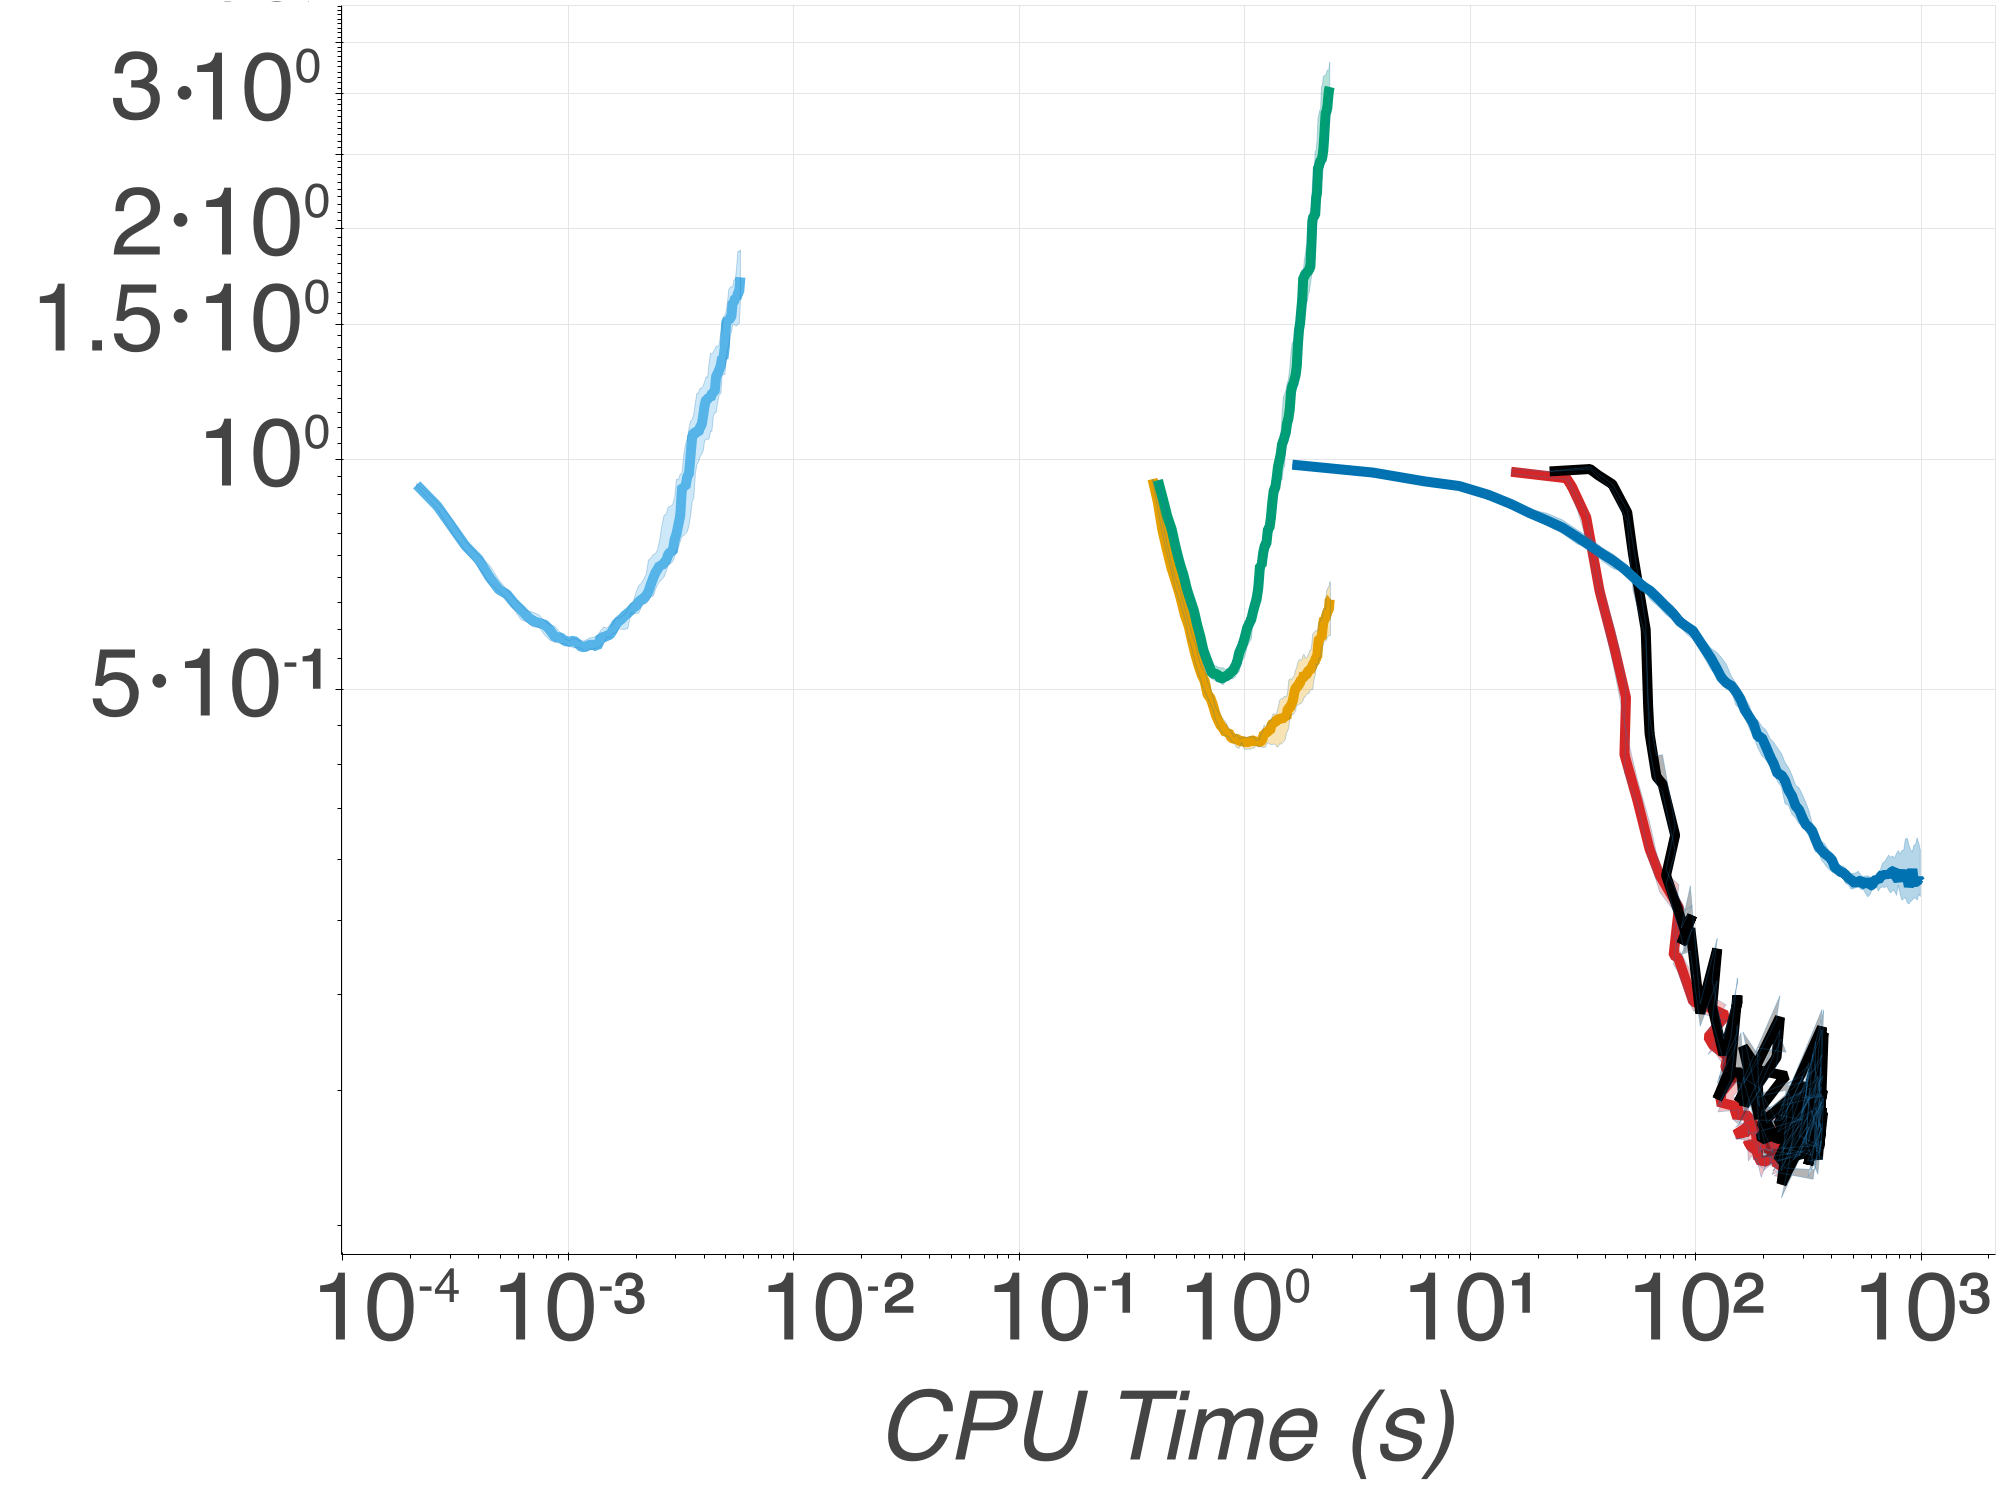
\includegraphics[width=1.15\columnwidth]{\MyPath/figs/wds1100_KLDvscput.png}}%
	\end{subfigure}\hfill\qquad
	\centering
	\begin{subfigure}[b]{.29\textwidth}
		\caption*{\textsc{Music}}
		\vspace*{-0.3cm}
		\centerline{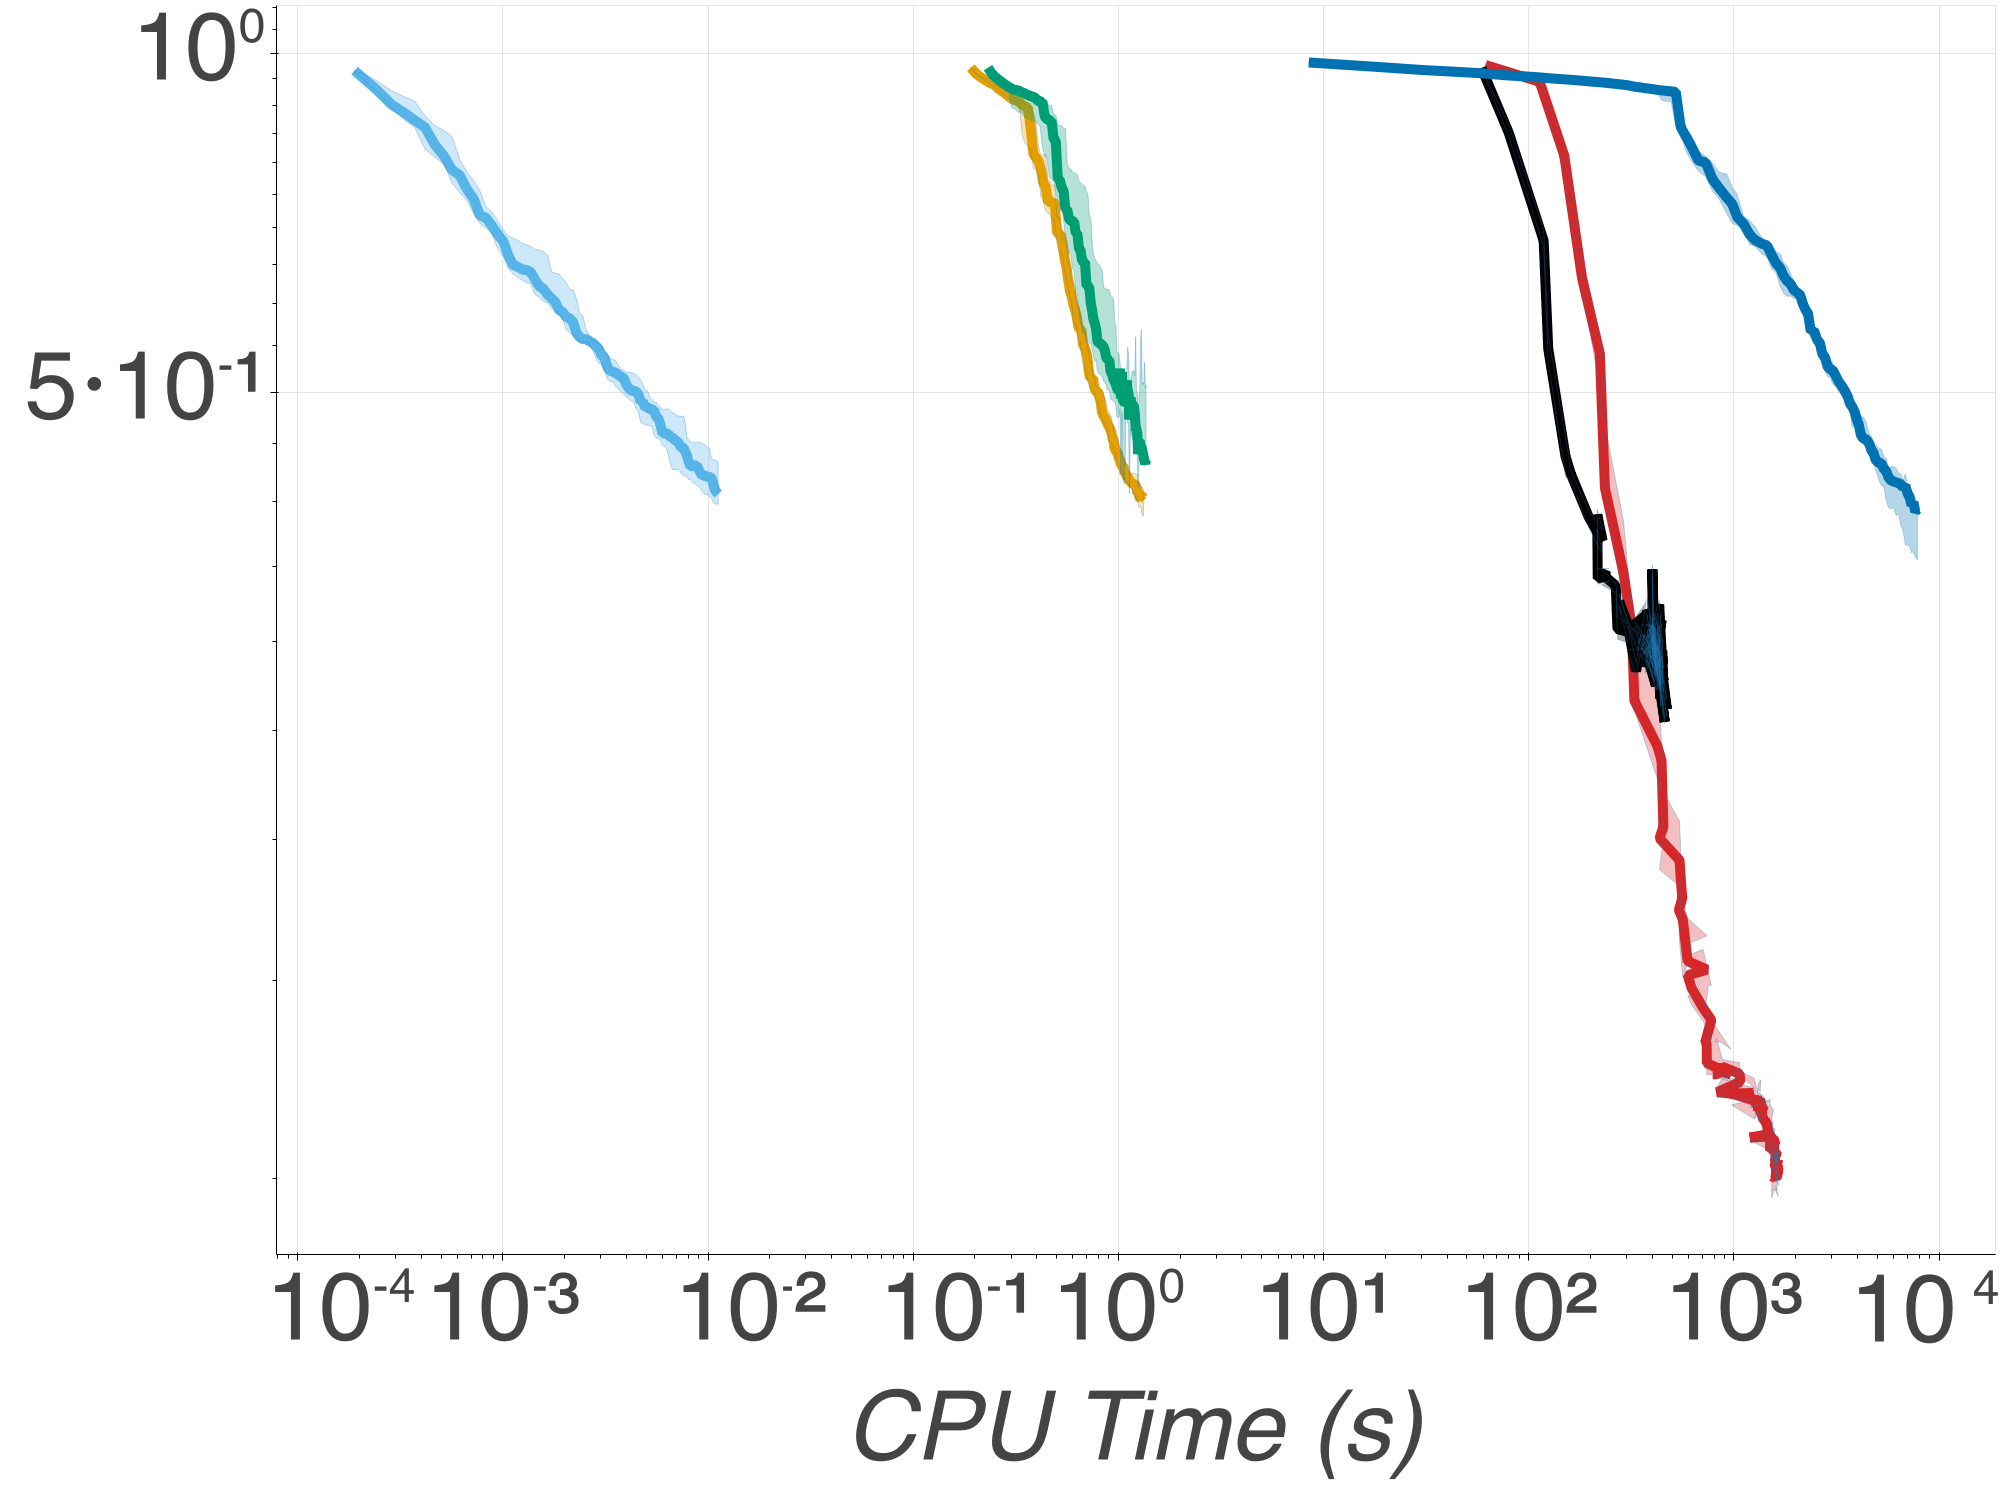
\includegraphics[width=1.15\columnwidth]{\MyPath/figs/wfma_KLDvscput.png}}%
	\end{subfigure}\hfill\qquad
	\caption{Comparison of \psvi~and \sparsevi~approximate posterior quality vs CPU time requirements for logistic regression experiment of~\cref{sec:experiments}.}
	\label{fig:30logreg_dkl_cput}
\end{figure*}

\begin{figure*}[!t]
	\centering
	\begin{subfigure}[b]{\textwidth}
		\centering
		\caption*{\textsc{Synthetic}}
		\vspace*{-0.3cm}
		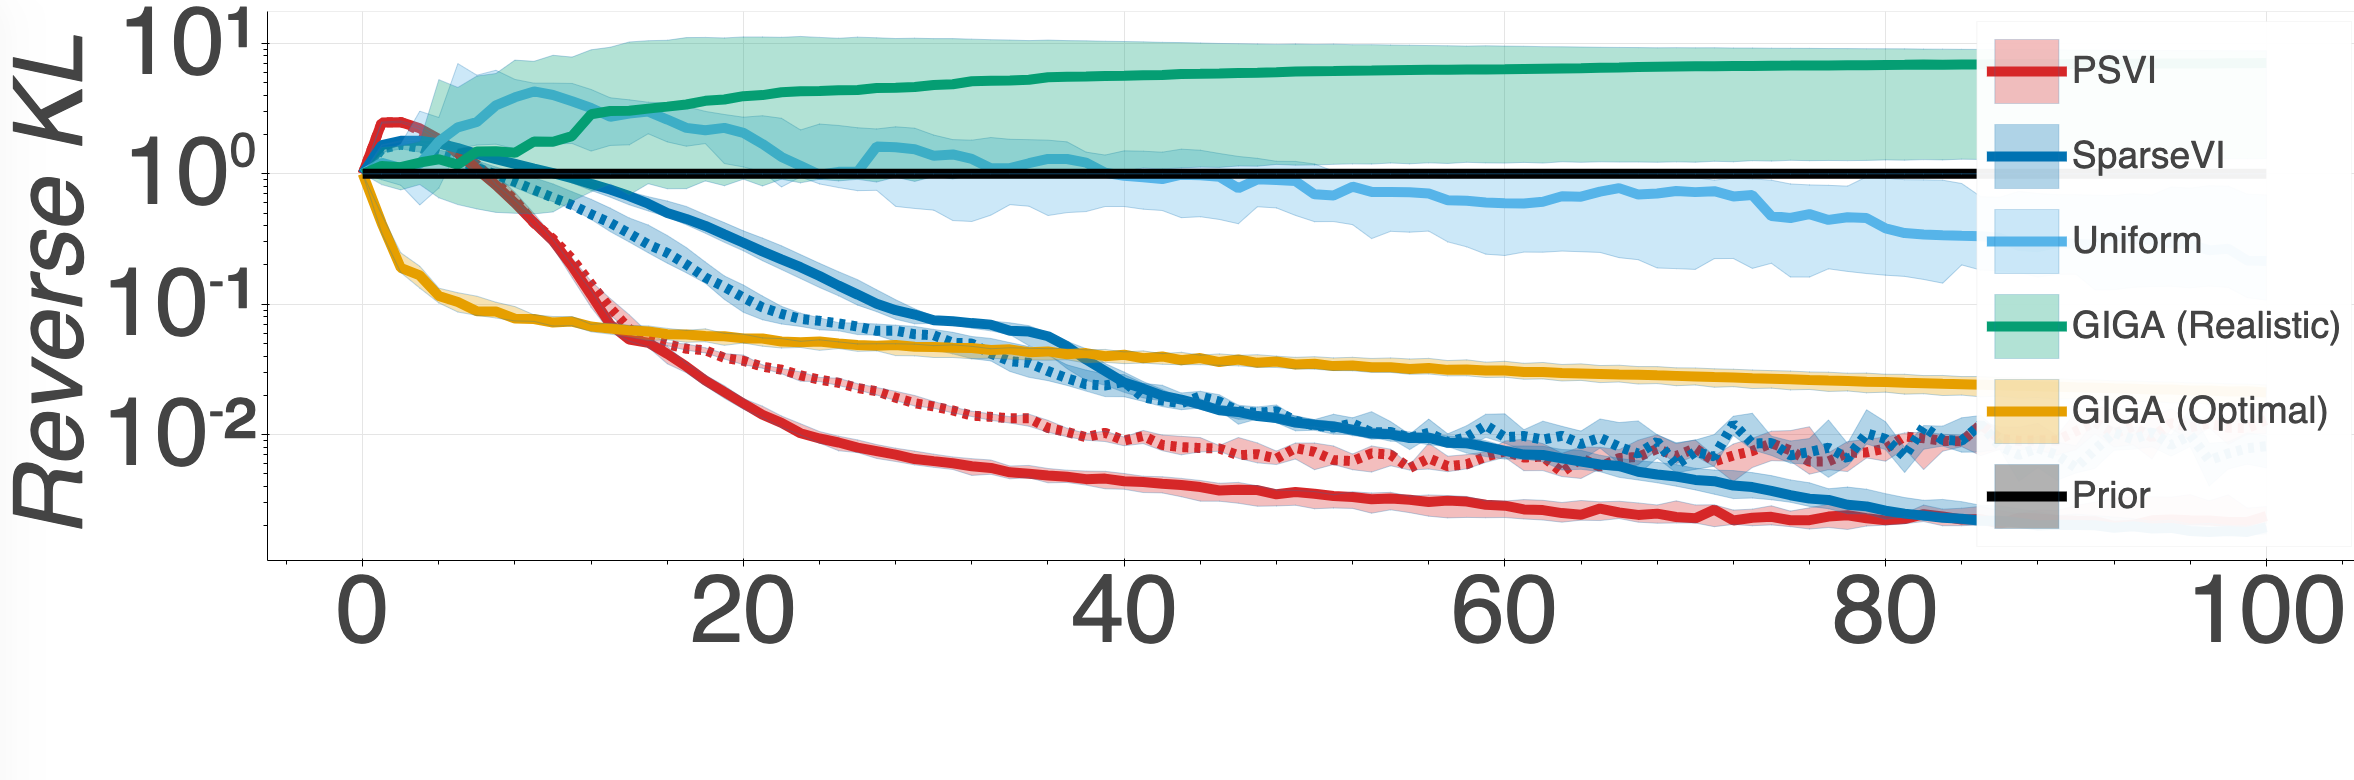
\includegraphics[width=0.495\textwidth, height=3.1cm]{\MyPath/tempfigs/synthlriter.png} \hfill 
		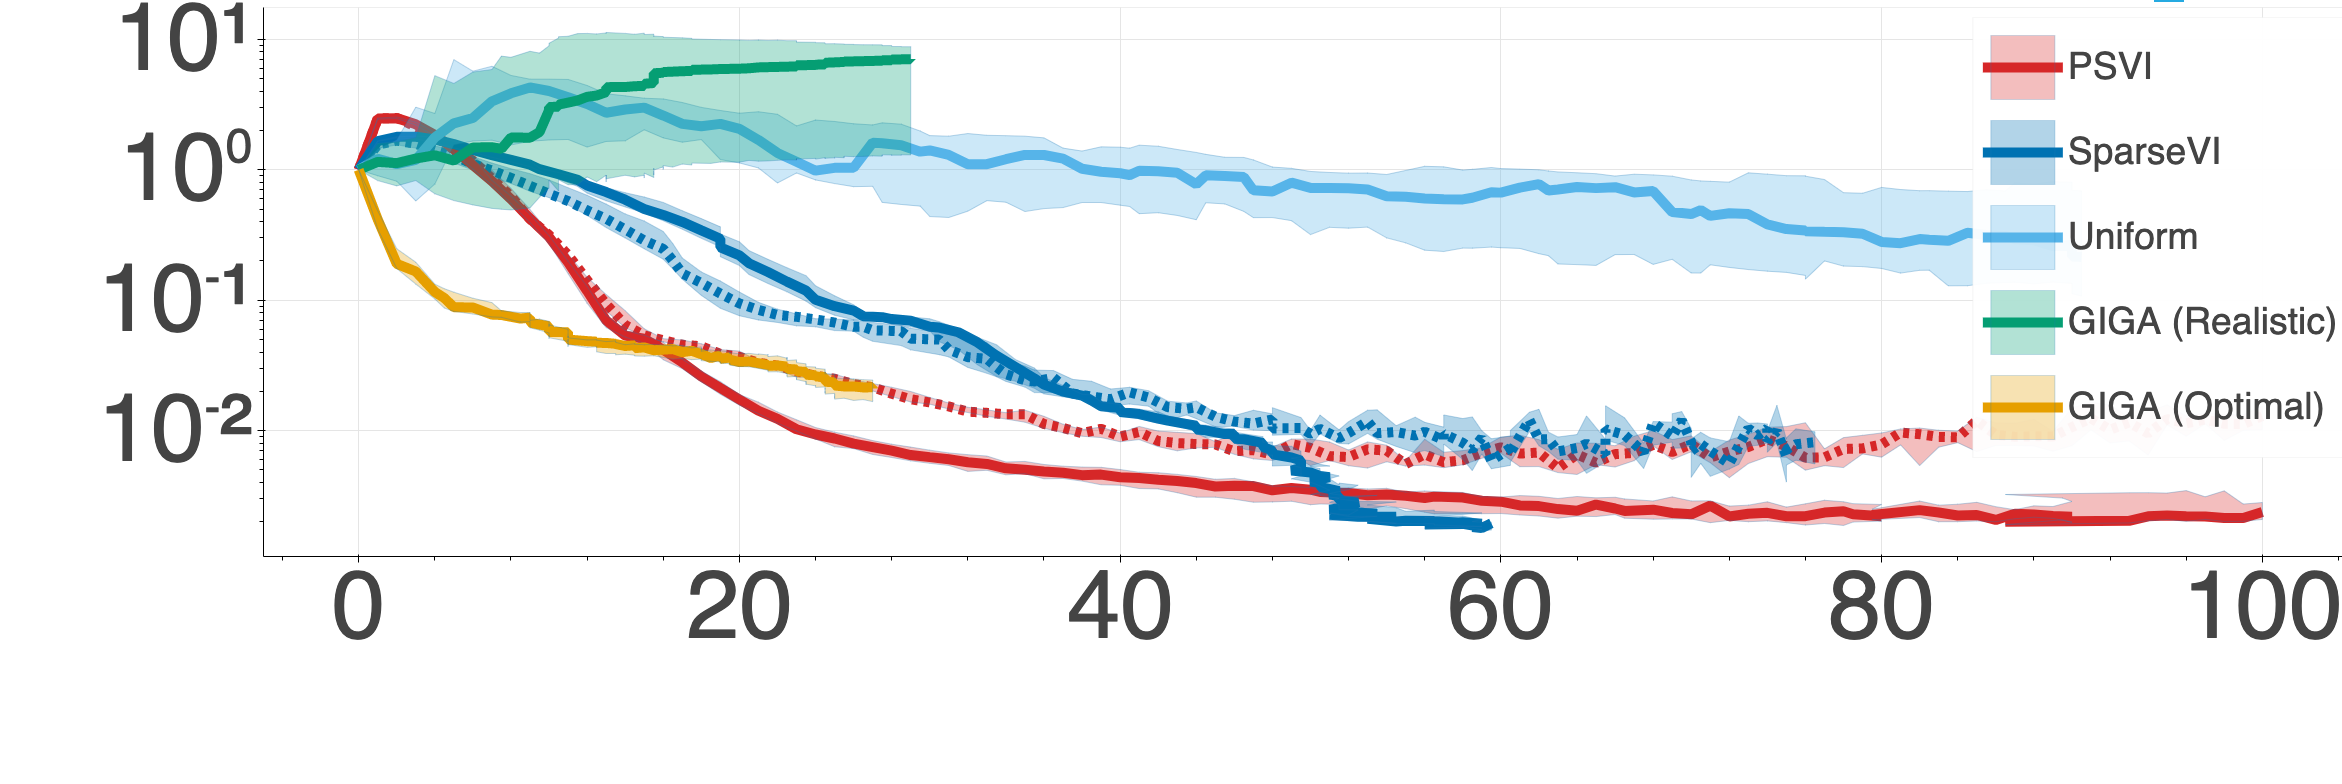
\includegraphics[width=0.495\textwidth, height=3.1cm]{\MyPath/tempfigs/synthlrsz.png}%
	\end{subfigure}\hfill\qquad
	\begin{subfigure}[b]{\textwidth}
		\centering
		\caption*{\textsc{Phishing}}
		\vspace*{-0.3cm}
		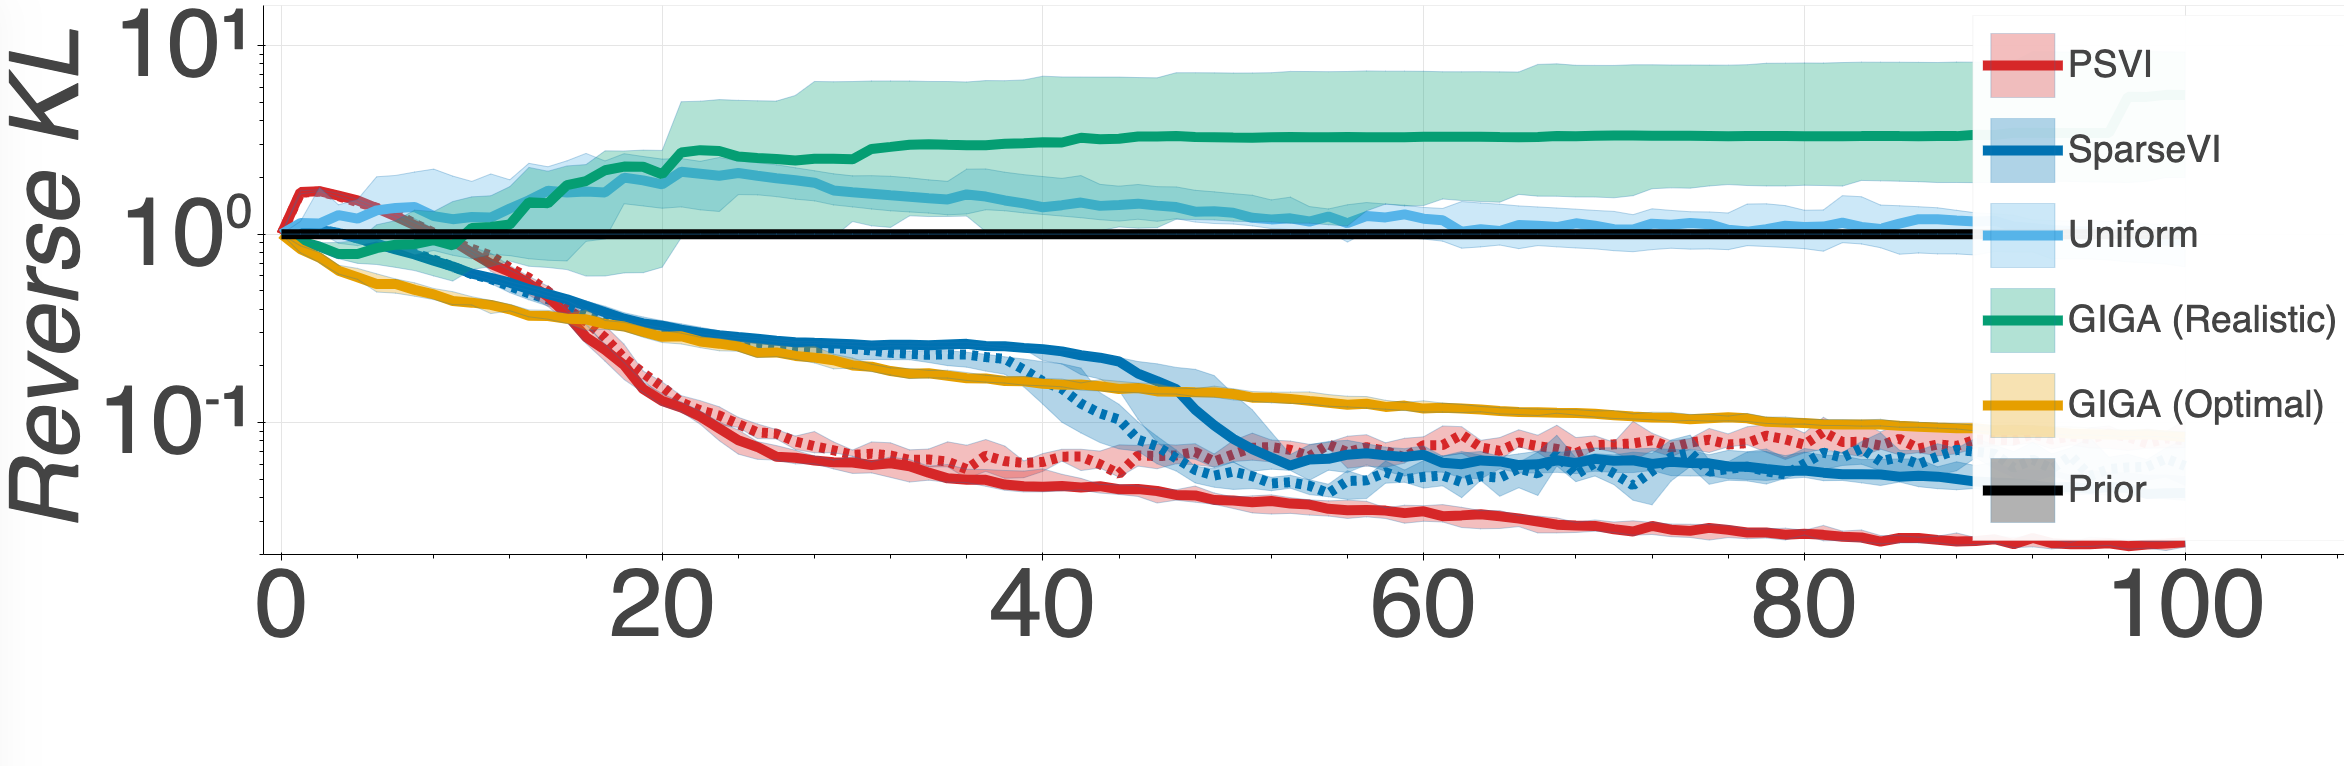
\includegraphics[width=0.495\textwidth, height=3.1cm]{\MyPath/tempfigs/phishingiter.png} \hfill
		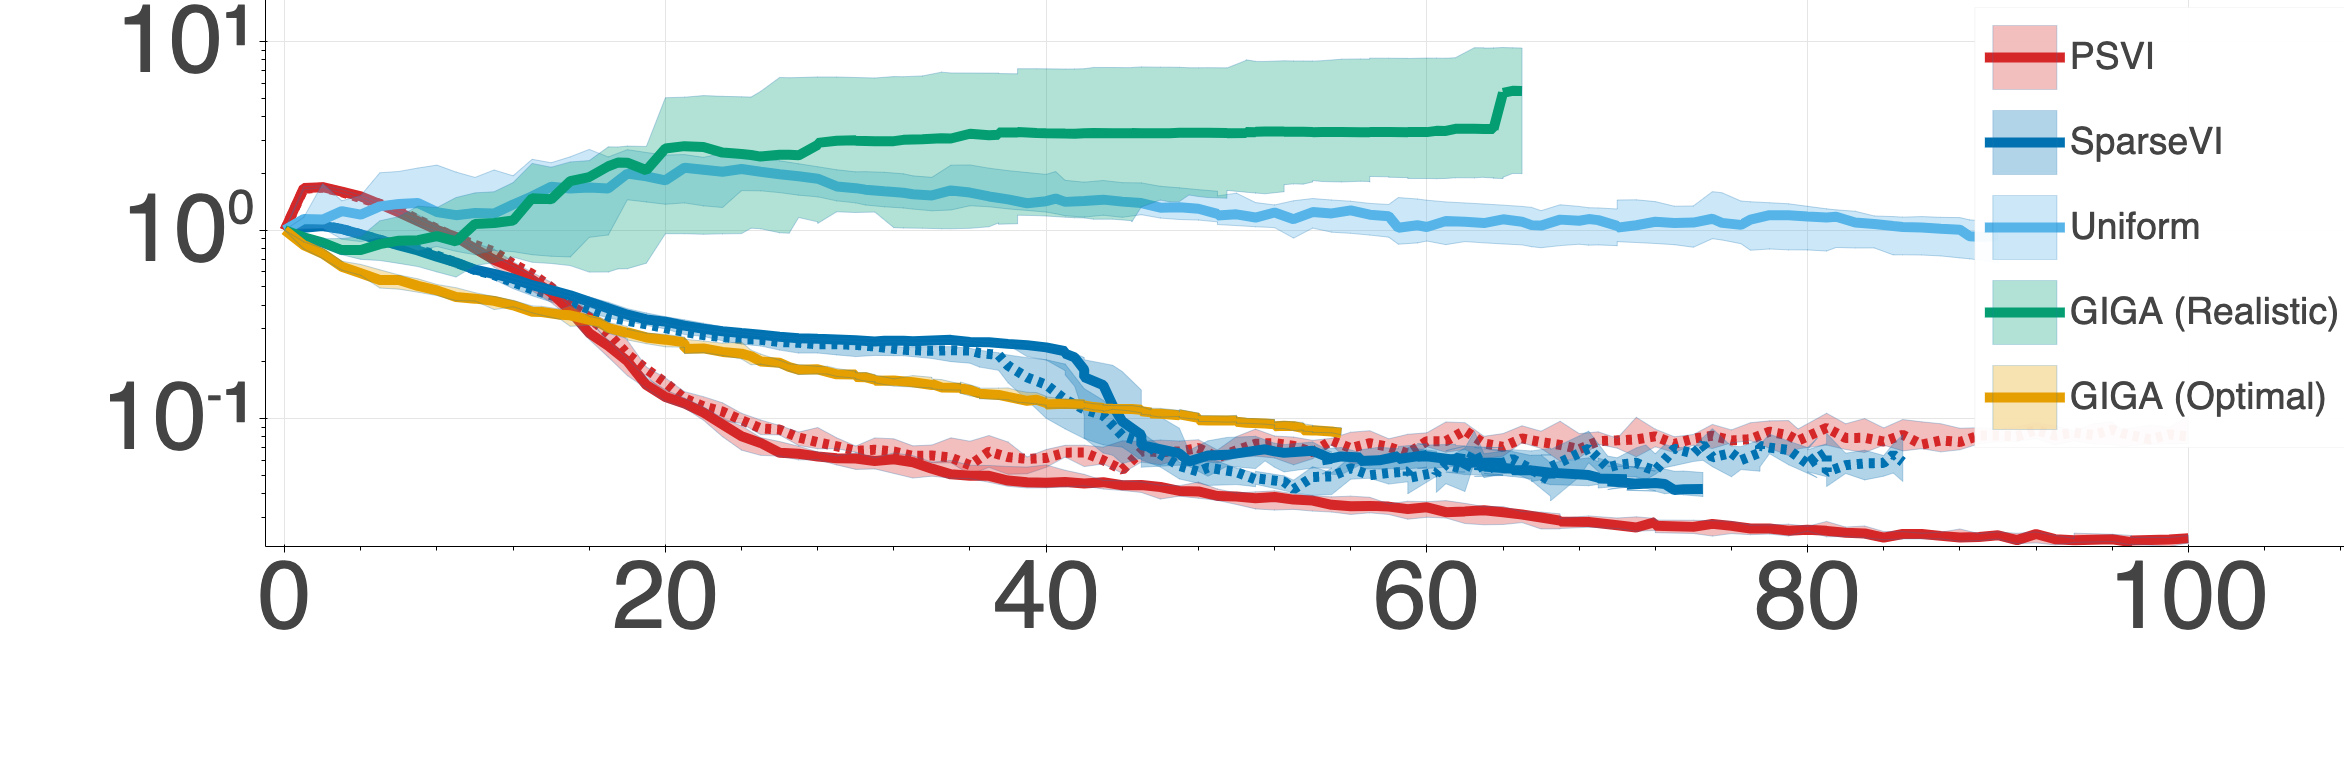
\includegraphics[width=0.495\textwidth, height=3.1cm]{\MyPath/tempfigs/phishingsz.png}%
	\end{subfigure}\hfill\qquad
	\begin{subfigure}[b]{\textwidth}
		\centering
		\caption*{\textsc{ChemReact}}
		\vspace*{-0.3cm}
		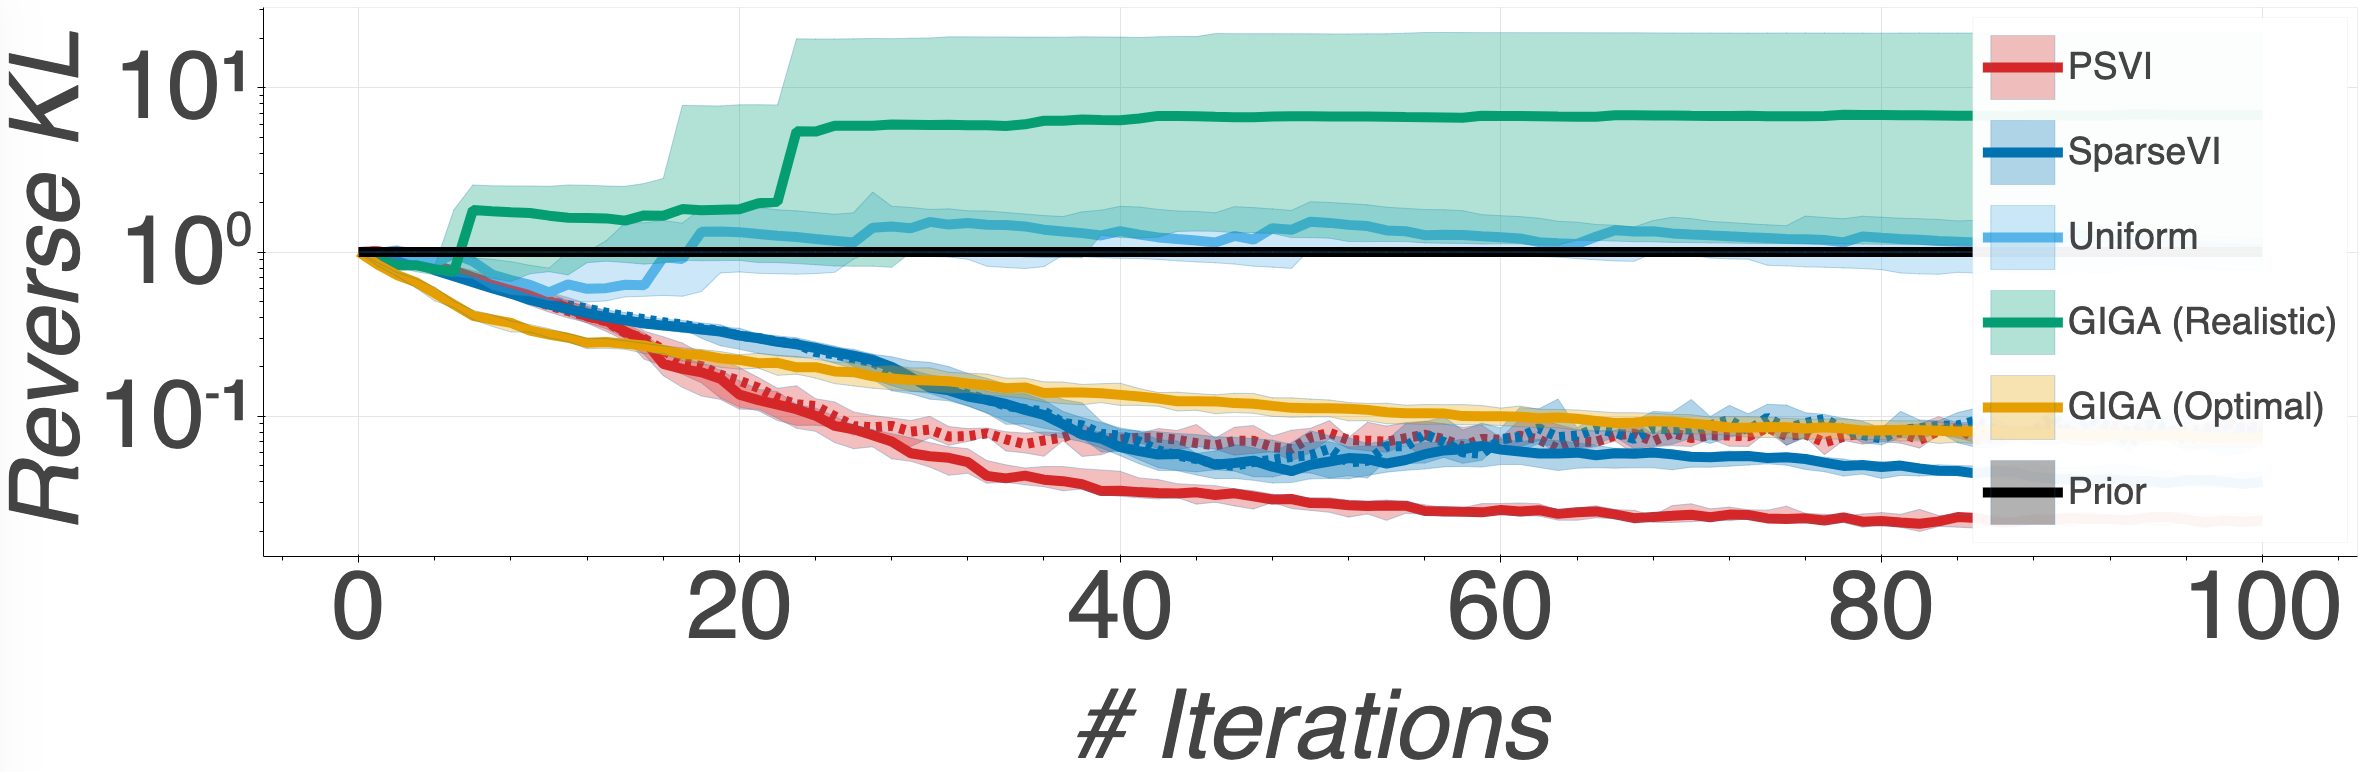
\includegraphics[width=0.495\textwidth, height=3.1cm]{\MyPath/tempfigs/ds1iter.png}
		\hfill
		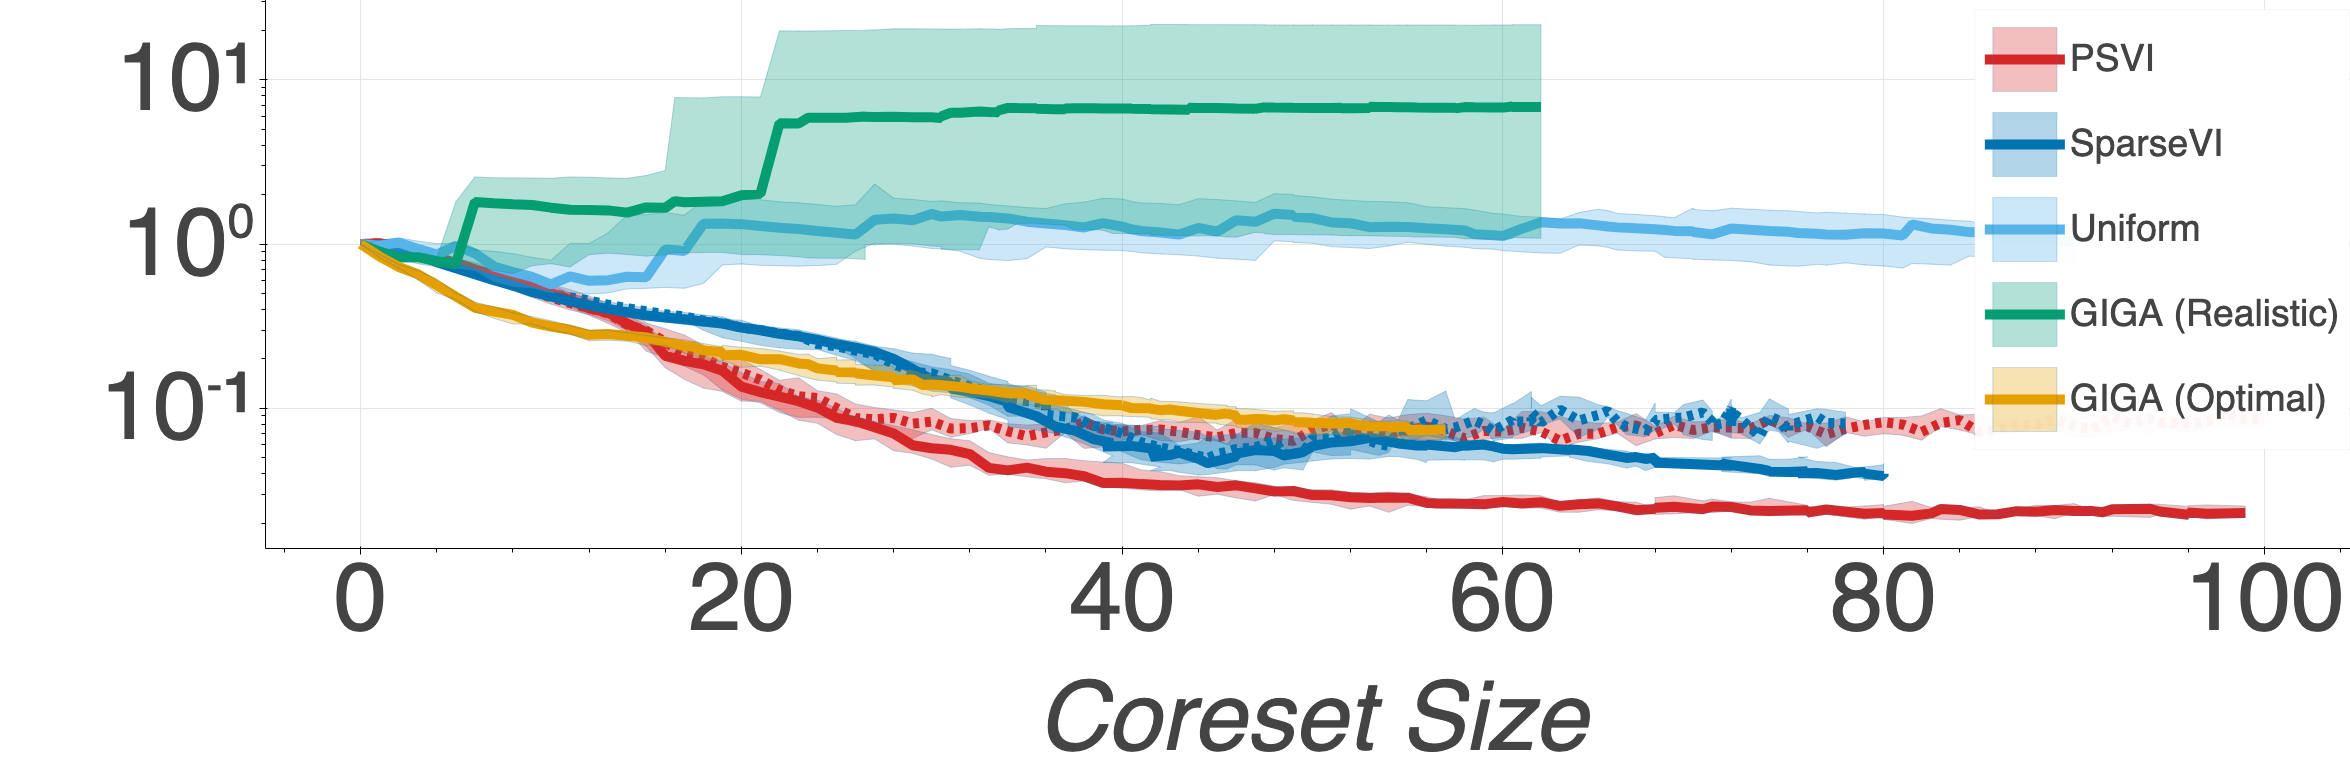
\includegraphics[width=0.495\textwidth, height=3.1cm]{\MyPath/tempfigs/ds1sz.png}%
	\end{subfigure}
	\caption{Comparison of incremental \psvi~and \sparsevi~approximate posterior
		quality vs iterations of incremental construction~(\emph{left}) and  coreset
		size~(\emph{right}) for logistic regression on small-scale experiment. With dashed lines is displayed the posterior quality achieved
		by incremental \psvi~and \sparsevi~constructions using gradients computed on random data subsets of size $256$.}
	\label{fig:logreg_dkl}
\end{figure*}

\paragraph{Evaluation of CPU time requirements} Experiments were performed on a CPU cluster node with a 2x Intel Xeon Gold 6142 and 12GB RAM. In the case of \psvi~the computation of coreset sizes from 1 to 100 was parallelized per single size over 32 cores in total. \cref{fig:30logreg_dkl_cput} shows posterior approximation error vs required CPU time for all coreset construction algorithms over logistic regression on the small-scale and large-scale datasets. As opposed to existing incremental coreset construction schemes, batch construction of \psvi~reduces the dependence between coreset size and processing cost: for \sparsevi~$\Theta(M^2)$ gradient computations are required, as this method builds up a coreset one point at a time; in contrast, \psvi~requires $\Theta(M)$ gradients since it learns all pseudodata points jointly. Although each gradient step of \psvi~is more expensive, practically this implies a steeper decrease in approximation error over processing time compared to \sparsevi. In the case of differentially private \psvi,~some extra CPU requirements are added due to the subsampled Gaussian mechanism computations.

\paragraph{Incremental scheme for pseudocoreset construction} We also experimented with an \emph{incremental scheme for pseudocoreset} construction. According to this scheme, pseudodata points are added sequentially to the pseudocoreset. Similarly to \sparsevi, in the beginning of each coreset iteration, we initialize a new pseudodata point at the true datapoint which maximizes correlation with current residual approximation error. Next, we jointly optimize the most recently added pseudodata point location, along with the pseudocoreset weights vector, over a gradient descent loop.  As opposed to batch construction, for large coreset sizes the incremental scheme for \psvi~does not achieve savings in CPU time compared to \sparsevi.

We evaluated coreset construction methods on Bayesian logistic regression. We used $M=100$ iterations for construction, $ S=100 $ Monte Carlo samples per gradient estimation, $ T= 100$ iterations for optimization, and learning rate $\gamma_t \propto 0.5t^{-1}$. Coreset posterior samples over the course of construction
for \sparsevi~and incremental \psvi~were drawn from a Laplace approximation using current
coreset weights and points. We implemented~\sparsevi~and incremental~\psvi~via computing gradients on the full dataset, as well as using stochastic gradients on subsets of size $B=256$ for lowering computational cost. 

Results presented in~\cref{fig:logreg_dkl} demonstrate that incremental \psvi~achieves consistently the smallest posterior approximation error, offering improvement
compared to \sparsevi~and even achieving better performance than \gigao. %, without the requirement for specifying a weighting function.  
We observe that stochastic gradients implementation~(dashed lines) reaches a plateau at higher values of KL compared to full gradients~(solid lines), but still achieves performance comparable with~\gigao.







